%\documentclass[10pt]{report} %twoside para impresion final 
\documentclass[11pt,a4paper]{report} %a4paper,

% Note: Make all your adjustments in here
%!TEX root = rdegiovanni-phd-tesis.tex
\usepackage[parts]{classicthesis} 

%\usepackage[left=1.5in,right=1.5in,top=1.5in,bottom=1.5in]{geometry} %configure margins
%\usepackage[left=3.65cm,right=3.65cm,bindingoffset=0.5cm]{geometry} %raul config

%%Options: Sonny, Lenny, Glenn, Conny, Rejne, Bjarne, Bjornstrup
%\usepackage[Bjarne]{fncychap}

\usepackage[T1]{fontenc}
% manual chapter style
%\newcommand\mychapterNumber{\normalfont\fontfamily{pplj}\fontsize{35}{36}\selectfont}
%\titleformat{\chapter}[block]%
%  {\vspace*{-2cm}}{\color{halfgray}\mychapterNumber\thechapter}{1em}
%  {\raggedright\spacedallcaps}[\normalsize\vspace*{.8\baselineskip}\color{halfgray}{\titlerule[2pt]}]%


% General useful packages
\usepackage[spanish, es-tabla, es-noquoting]{babel}
\usepackage{amsmath,amsthm,amssymb,verbatim}
\usepackage{graphicx}
\usepackage{caption}
\usepackage{subcaption}
\usepackage{alltt}
\renewcommand{\ttdefault}{txtt}
\usepackage{mathrsfs}
\usepackage{stmaryrd}
%\usepackage[hidelinks]{hyperref}
\usepackage{enumitem}
\usepackage{proof}
\usepackage{lscape}
\usepackage{booktabs}
\usepackage{tikz}
\usetikzlibrary{matrix,chains,positioning,calc,shadows,fit,arrows, shapes, shapes.geometric, petri} 
\usetikzlibrary{decorations.text, decorations.markings,decorations.pathreplacing} %calc,decorations.pathmorphing}
%\usetikzlibrary{shapes,fit,arrows,calc,positioning, decorations.pathreplacing}

%citations
\usepackage[hyperpageref]{backref}
\usepackage{cite}
\renewcommand\citepunct{; }

%paragraph space
\setlength{\parskip}{.2cm}%\baselineskip}

% import tikz styles
%\input{LTS-style}

% listings
\usepackage{listings}
\definecolor{lightgray}{gray}{.60}
\definecolor{Lightgray}{gray}{.98}
\definecolor{bordegray}{gray}{.70}
\definecolor{gray}{gray}{.3}

% Hyperreferences
\hypersetup{%
    %draft,	% = no hyperlinking at all (useful in b/w printouts)
    colorlinks=true, linktocpage=true, pdfstartpage=3, pdfstartview=FitV,%
    % uncomment the following line if you want to have black links (e.g., for printing)
    %colorlinks=false, linktocpage=false, pdfborder={0 0 0}, pdfstartpage=3, pdfstartview=FitV,% 
    breaklinks=true, pdfpagemode=UseNone, pageanchor=true, pdfpagemode=UseOutlines,%
    plainpages=false, bookmarksnumbered, bookmarksopen=true, bookmarksopenlevel=1,%
    hypertexnames=true, pdfhighlight=/O,%nesting=true,%frenchlinks,%
    urlcolor=webbrown, linkcolor=RoyalBlue, citecolor=gray!20!RoyalBlue %webgreen, %pagecolor=RoyalBlue,%
    %urlcolor=Black, linkcolor=Black, citecolor=Black, %pagecolor=Black,%
}


% References
\usepackage[spanish]{cleveref}
\crefname{figure}{Figura}{Figuras}
\crefname{table}{Tabla}{Tablas}
\crefname{chapter}{Cap\'itulo}{Cap\'itulos}
\crefname{section}{Secci\'on}{Secciones}
\crefname{subsection}{Subsecci\'on}{Subsecciones}
\crefname{definition}{Definici\'on}{Definiciones}
\crefname{theorem}{Teorema}{Teoremas}
\crefname{lemma}{Lema}{Lemas}
\crefname{algorithm}{Algoritmo}{Algoritmos}
%\renewcommand{\figureautorefname}{Figura}%
%\renewcommand{\figureautorefname}{Figura}%
%\renewcommand{\tableautorefname}{Tabla}%
%\renewcommand{\partautorefname}{Parte}%
%\renewcommand{\chapterautorefname}{Cap\'itulo}%
%\renewcommand{\sectionautorefname}{Secci\'on}%
%\renewcommand{\subsectionautorefname}{Secci\'on}%
%\renewcommand{\subsubsectionautorefname}{Secci\'on}% 	
%\renewcommand{\listtablename}{\'Indice de Tablas}
% ********************************************************************
% Using different fonts
% ********************************************************************
%\usepackage[oldstylenums]{kpfonts} % oldstyle notextcomp
%\usepackage[osf]{libertine}
%\usepackage{hfoldsty} % Computer Modern with osf
%\usepackage[light,condensed,math]{iwona}
%\renewcommand{\sfdefault}{iwona}
\usepackage{lmodern} % <-- no osf support :-(
%\usepackage[urw-garamond]{mathdesign} <-- no osf support :-(
% ****************************************************************************************************

% Personal data and user ad-hoc commands
\newcommand{\ingles}[1]{#1}
\newcommand{\lenguaje}[1]{{\sc#1}}
\newcommand{\herramienta}[1]{\textsf{#1}}
\newcommand{\codigo}[1]{\texttt{#1}}
\newcommand{\FSPcode}[1]{\colorbox{gray!10}{\textcolor{black}{\tt #1}}}
\newcommand{\ALVcode}[1]{\colorbox{gray!10}{\textcolor{black!80}{\tt #1}}}

% Teoremas, Lemas, Definiciones y Ejemplos
\newtheorem{theorem}{Teorema}[chapter]
\newtheorem{lemma}[theorem]{Lema}
\newtheorem{definition}{Definici\'on}[chapter]
\newtheorem{example}{Ejemplo}[chapter]


\newcommand{\tituloES}{Expresiones de navegaci\'on, el mutante perdido.}

\newcommand{\HRule}{\rule{\linewidth}{0.5mm}}

%%% 
\newcommand{\SAT}[1]{\models_{\scriptscriptstyle{#1}}}
\newcommand{\LTSproc}[1]{\textbf{\texttt{#1}}}
\newcommand{\Fluent}[1]{\textit{#1}}

\newcommand{\GoalDef}[1]{\fbox{\parbox{\textwidth}{#1}}}

%% Algoritmos
\usepackage[chapter]{algorithm}
\usepackage[noend]{algpseudocode}
% New definitions
\algnewcommand\algorithmicswitch{\textbf{switch}}
\algnewcommand\algorithmiccase{\textbf{case}}
\algnewcommand\algorithmicassert{\texttt{assert}}
\algnewcommand\Assert[1]{\State \algorithmicassert(#1)}%
% New "environments"
\algdef{SE}[SWITCH]{Switch}{EndSwitch}[1]{\algorithmicswitch\ #1\ \algorithmicdo}{\algorithmicend\ \algorithmicswitch}%
\algdef{SE}[CASE]{Case}{EndCase}[1]{\algorithmiccase\ #1}{\algorithmicend\ \algorithmiccase}%
\algtext*{EndSwitch}%
\algtext*{EndCase}%
\newcommand{\Break}{\State \textbf{break} }
\newcommand{\Continue}{\textbf{continue} }
%\algnewcommand{\LineComment}[1]{\State \algorithmicend\ right\) #1}
\algnewcommand{\LineComment}[1]{\State {\small \(--\) #1}}
\algnewcommand{\MyComment}[1]{{\small \(--\) #1}}
%\newcommand{\Let}{\State \textbf{let} }
\algblockdefx{Let}{EndLet}[1]{\textbf{let} #1 \textbf{in}}{\textbf{endlet}}
\algtext*{EndLet}%


\begin{document}
\frenchspacing
\raggedbottom

% ********************************************************************
% Frontmatter
\pagenumbering{roman}
\pagestyle{plain}
%\include{titlepage}
%!TEX root = rdegiovanni-phd-tesis.tex
\begin{titlepage}

\begin{center}
{\LARGE \textbf{Mutaci\'on de Expresiones de Navegaci\'on para Testing y Reparaci\'on}}\\ 
\vspace{4mm}
{\Large por Sim\'on Emmanuel Guti\'errez Brida}\\

\vspace{50mm}

Presentado ante la Facultad de Matem\'atica, Astronom\'ia y F\'isica\\
como parte de los requerimientos para la obtenci\'on del grado de\\
Doctor en Ciencias de la Computaci\'on de la\\
\textsc{Universidad Nacional de C\'ordoba}\\
 
\vspace{50mm}

Noviembre, 2018\\
@FaMAF - UNC 2018\\
{\Large Director: Nazareno Mat\'ias Aguirre}

\vspace{10mm}
\href{https://licensebuttons.net/l/by-nc-sa/4.0/88x31.png}{
\includegraphics{images/licencia-famaf.png}}\\
{Mutaci\'on de Expresiones de Navegaci\'on para Testing y Reparaci\'on por Sim\'on Emmanuel Guti\'errez Brida se distribuye bajo una \href{https://creativecommons.org/licenses/by-nc-sa/4.0/deed.es_ES}{Licencia Creative Commons Atribución-NoComercial-CompartirIgual 4.0 Internacional}.}
\end{center}  
\end{titlepage} 

%LICENCIA FAMAF
%<a rel="license" href="http://creativecommons.org/licenses/by-nc/2.5/ar/"><img alt="Licencia Creative Commons" style="border-width:0" src="https://i.creativecommons.org/l/by-nc/2.5/ar/88x31.png" /></a><br /><span xmlns:dct="http://purl.org/dc/terms/" property="dct:title">Técnicas Automáticas para la Elaboración, Validación y Verificación de Requisitos de Software</span> por <a xmlns:cc="http://creativecommons.org/ns#" href="http://dc.exa.unrc.edu.ar/staff/rdegiovanni/" property="cc:attributionName" rel="cc:attributionURL">Renzo Degiovanni</a> se distribuye bajo una <a rel="license" href="http://creativecommons.org/licenses/by-nc/2.5/ar/">Licencia Creative Commons Atribución-NoComercial 2.5 Argentina</a>.


%\textbf{Lugar de Trabajo}
% Departamento de Computaci\'on\\
%\hspace{3cm} Facultad de Ciencias Exactas F\'isico-Qu\'imicas y Naturales\\
%\hspace{3cm} Universidad Nacional de R\'io Cuarto\\
%\vspace{5mm}
%Director: \textbf{Dr.~Nazareno~Mat\'ias~Aguirre}\\
%\vspace{5mm}
%Jurado:\\
%\vspace{5mm}
%\noindent
%C\'ordoba, Argentina, 2014


\cleardoublepage\null
%!TEX root = main.tex
\chapter*{Resumen}
Verificar que un sistema de \emph{software} realiza correctamente las tareas para las cuales fue desarrollado es una de las actividades de mayor importancia en \emph{Ingenier\'ia de Software}, y concentra un significativo esfuerzo de investigaci\'on en esta \'area. El \emph{testing}, el cual consiste en ejecutar el programa a evaluar en un conjunto de escenarios particulares y contrastar el comportamiento esperado con el obtenido, es una de las t\'ecnicas m\'as utilizadas, como forma de comprobaci\'on del correcto comportamiento del software.

Dada la inherente incompletitud de \emph{testing}, una selecci\'on de los escenarios bajos los cuales realizar la evaluaci\'on, es necesaria. Claramente, c\'omo \'esta es realizada va a afectar la confianza que genere, cuando la ejecuci\'on real del software coincida con la esperada, es decir, que el conjunto seleccionado sea un buen representante de todos los posibles escenarios. Los criterios de testing permiten medir la calidad de un conjunto de tests generando objetivos a ser cubiertos, y evaluando cu\'antos de estos son satisfechos (cubiertos) por los tests. \emph{Mutation testing} es uno de estos, y consiste en inyectar fallas artificiales en el software bajo evaluaci\'on, y evaluar la capacidad de detecci\'on, por parte de los tests, de estas fallas.

Las fallas generadas por mutation testing se basan en operadores de mutaci\'on, las cuales deben ser buenos representantes de fallas reales, tradicionalmente generando cambios simples, tales como el reemplazo de operadores aritm\'eticos y relacionales. Estudios recientes han demostrado la falta de representaci\'on para ciertas fallas reales, incluso por operadores considerados \emph{suficientes}, principalmente en el contexto de programaci\'on orientada a objetos, usualmente obviada por los operadores actuales, motivando el desarrollo de nuevos operadores.

En esta tesis presentaremos un nuevo operador de mutaci\'on que aplica a expresiones de navegaci\'on, un tipo de expresiones muy utilizadas en programas orientados a objetos. Daremos una definici\'on formal del mismo, evaluando su aplicaci\'on en el contexto de \emph{mutation testing} y reparaci\'on de programas. Bajo principalmente colecciones implementadas en lenguajes orientados a objetos, mostraremos la producci\'on de fallas y generaci\'on de reparaciones no previamente representadas.

\noindent
\textbf{Palabras Clave:} Ingenier\'ia de Software, Mutaci\'on, Operadores de Mutaci\'on, Expresiones de navegaci\'on.







\cleardoublepage%\null
%%!TEX root = main.tex
\chapter*{Agradecimientos}
Mam\'a, Pap\'a, ten\'ian raz\'on, Microbiolog\'ia no era lo m\'io. Gracias por el aguante!.

Naza, gracias por la paciencia, desde alumno que no era f\'acil, as\'i que me imagino lo que debe haber sido bancarme hasta el doctorado. Finalmente termin\'e aprendiendo a mantenerme en el camino durante un trabajo de investigaci\'on, sin tu constancia no lo hubiera logrado. Aprend\'i y sigo aprendiendo mucho de vos, gracias por estar siempre.

Mis amigos del DC, fueron varios a\~nos que se pasaron volando, tuve la suerte de trabajar junto a varios de ustedes y me ayudaron mucho durante el doctorado. Marcelo, gracias por todas las veces que me ayudaste con mis intento de magia negra en Java; Germ\'an, dejarme participar como tester en varios proyectos me dej\'o aprender a no complicarme tanto; Gast\'on, te sumaste a trabajar conmigo en un paper incluso cuando solo ten\'iamos una semana disponible; Pablo, te toc\'o tenerme al lado en la oficina y me bancaste las 1001 preguntas que te hice; Renzo y Vale, me ayudaron a tranquilizarme cuando estaba en la recta final; Sonia y Marta, gracias por la paciencia, malcriarme un poco, y ense\~narme tanto desde que empec\'e la carrera. A todos, gracias por su amistad.

No hay suficiente lugar para agradecer con todos los detalles que merecen a todos los que me acompa\~naron, pero quiero simplemente terminar con un gracias.

\cleardoublepage
%\newpage
%\topskip0pt
\vspace*{7cm}
\hfill {\Large ``No somos nada.''}
%\cleardoublepage
%\tableofcontents
%\cleardoublepage
%\listoffigures
%\cleardoublepage
%\listoftables
\pagestyle{scrheadings}
%\cleardoublepage
% ********************************************************************
% Mainmatter
\pagestyle{headings}
\pagenumbering{arabic}
%\part{?`Porqu\'e la Ingenier\'ia de los Requisitos de Software?} %\ctparttext{text}
\cleardoublepage
%!TEX root = main.tex
\chapter{Introducci\'on}
\label{cap:introduccion}

En la actualidad, el software se encuentra en todos los aspectos de la vida diaria, y en general la expectativa del usuario es confiar en que el mismo simplemente funciona. Nadie espera que el autom\'ovil no arranque por un error en el software embebido que utiliza, o que el cajero autom\'atico de un banco no retorne billetes al realizar una extracci\'on v\'alida, o que el reloj del tel\'efono celular marque un horario incorrecto, etc. Sin embargo, son innumerables los ejemplos de errores de software, que causan comportamientos indebidos del mismo. Algunos de estos errores pueden ser catastr\'oficos. Algunos ejemplos son los siguientes. En 2015 se descubri\'o un bug en el modelo Boeing 787 Dreamliner que pod\'ia causar el apagado de todos los generadores el\'ectricos del avi\'on, si \'este permanec\'ia encendido por m\'as de 248 d\'ias. En los a\~nos 80, un error en el c\'odigo del controlador para la m\'aquina de terapia de radiaci\'on \emph{Therac-25}, caus\'o la muerte de varios pacientes al administrar cantidades excesivas de radiaci\'on beta. En 2018 un bug en WhatsApp causaba que la aplicaci\'on, y en muchos casos el dispositivo, dejara de responder, si se recib\'ia un mensaje en Unicode, conteniendo una secuencia que repet\'ia el caract\'er especial que especifica la direcci\'on de renderizado del texto.
%REF: BUG AVION: https://s3.amazonaws.com/public-inspection.federalregister.gov/2015-10066.pdf
%REF: THREAC-25, CITATION NEEDED?
%REF: BLACK DOT OF DEATH, CITATION NEEDED?

Claramente, suponer que el software simplemente funciona, es un error. Los errores en un programa pueden tener consecuencias que van desde una molestia menor al usuario, hasta la p\'erdida de vidas. Esto muestra la enorme relevancia del problema de garantizar la correcci\'on de un programa, es decir, la comprobaci\'on de que para todo escenario de uso, incluyendo las entradas directas e indirectas del software, el programa se comporta como se espera, o equivalentemente arroja el resultado esperado. Uno de los enfoques tradicionales, y de mayor adopci\'on en la pr\'actica, para analizar la correcci\'on de un programa es el \emph{testing}, que consiste en evaluar el comportamiento del programa en cuesti\'on en un conjunto espec\'ifico de escenarios de ejecuci\'on. Dado que la comprobaci\'on exhaustiva de todos los escenarios de ejecuci\'on es en general inviable salvo para programas muy simples, en la pr\'actica s\'olo un subconjunto de estos escenarios puede ser evaluado. Cu\'antos y cu\'ales de todos los escenarios se seleccionan est\'a directamente relacionado con la confianza que brindar\'a el proceso de testing, en caso de no encontrar fallas, de que el software funciona correctamente.

% No va aca
%No solamente es necesario un conjunto de escenarios, el comportamiento esperado requiere ser definido, y la forma m\'as simple es usando un valor esperado, por ejemplo, esperar que llamar a un m\'etodo \texttt{helloWorld()} retorne la cadena \emph{"Hello World"}; un ejemplo m\'as complejo es que luego de ejecutar el m\'etodo \texttt{insert(3)} sobre una lista vac\'ia, llamar al m\'etodo \texttt{contains(3)} retorne verdadero. Otra forma de evaluar el comportamiento esperado es evaluando propiedades, como un orden ascendente de los elementos en una lista simplemente encadenada, antes y despu\'es de ejecutar cualquier m\'etodo sobre la misma. Lo que define el comportamiento esperado es lo que se conoce como \emph{Or\'aculo}.

% No va aca
%Podemos entonces definir a un test, como una serie de pasos conteniendo tres partes principales: \emph{Preparaci\'on}(Arrange), consiste en definir o construir el escenario sobre el que se va a evaluar un programa; \emph{Ejecuci\'on}(Act), donde se va a ejecutar el programa a evaluar; \emph{Evaluaci\'on}(Assert), donde se va a evaluar el resultado obtenido contra el esperado.

Un conjunto de tests (los escenarios de ejecuci\'on del software bajo an\'alisis) debe ser necesariamente finito, lo cual implica que en general no es posible en la pr\'actica evaluar exhaustivamente una pieza de software en todos los posibles escenarios de ejecuci\'on. M\'as a\'un, la ejecuci\'on del software en los escenarios elegidos debe insumir recursos razonables; esto por supuesto va a depender del contexto y los recursos disponibles, pero en l\'ineas general es esperable que la ejecuci\'on de los casos de tests sea \emph{eficiente}, especialmente aquellos que el desarrollador utiliza como apoyo constante a sus actividades de programaci\'on. 

%No va aca
%finalmente el \'exito en la execuci\'on de estos tests, es decir, que ninguno detecte una diferencia entre el resultado obtenido y el esperado, deber\'ia servir como control de calidad del software.

Dado que la finalidad de testing es evaluar un programa en un subconjunto de todos sus escenarios posibles, como forma aproximada de estimar (a trav\'es de una generalizaci\'on) su correcto comportamiento en el universo de todos los escenarios de ejecuci\'on, es necesario contar con un criterio para evaluar la calidad del conjunto elegido, es decir, evaluar cu\'an bien un conjunto de escenarios representa el universo de \'estos. Intuitivamente, un buen conjunto de casos de tests, o \emph{test suite}, es aquel que tiene una alta capacidad de detectar fallas: si existe un bug en el programa, alg\'un test en la suite es capaz de detectarlo. Sin embargo, esta intuici\'on, como criterio para evaluar cu\'an buena es una suite, es viable s\'olo si uno conoce de antemano los bugs del programa bajo an\'alisis. 
% No tiene sentido aca, y no se entiende
%La raz\'on de esto es que las fallas se definen en t\'erminos de su reparaci\'on, por ejemplo, \emph{falta incrementar la variable \texttt{i} al recorrer el arreglo}, no solo eso, sin\'o que se define en base a \emph{una} posible reparaci\'on, cuando en general, \'estas son infinitas. 
Resulta necesario entonces utilizar criterios indirectos, para medir la calidad de suites de tests. Estos criterios definen en general metas o requisitos a cubrir por los tests, a partir de los cuales se puede \emph{medir} cu\'antos son efectivamente cubiertos. Estos criterios de evaluaci\'on se suelen dividir en dos categor\'ias principales: \emph{caja blanca} (white box), cuando las metas a cubrir se basan en la estructura del programa, y \emph{caja negra} (black box), cuando las metas se basan en las especificaciones. Algunos ejemplos t\'ipicos de citerios de caja blanca son la \emph{cobertura de sentencias}, que exige ejecutar a trav\'es de la suite todas las sentencias en un programa, y \emph{cobertura de ramas}, que exige ejecutar todas las alternativas para las sentencias de control de flujo. Determinar clases de equivalencia para las entradas del programa basado en su especificaci\'on, y tener al menos un escenario por cada una de estas clases, es un ejemplo de un criterio de caja negra (denominado \emph{particionado en clases de equivalencia}).

Un ejemplo de c\'omo los criterios de evaluaci\'on de test suites intentan dar una medida indirecta de la capacidad de las mismas en detectar fallas potenciales se puede apreciar en la cobertura de sentencias. Este criterio impone, como metas a cubrir, la ejecuci\'on de cada una de las sentencias del programa bajo evaluaci\'on. La intuici\'on de este criterio es bastante simple: lo m\'inimo indispensable para descubrir una falla, es ejecutar la sentencia o sentencias donde se encuentra el defecto asociado a la misma. Es sin embargo f\'acil encontrar ejemplos de fallas simples donde este criterio da una evaluaci\'on positiva a un conjunto de tests, y a\'un as\'i es incapaz de detectar fallas. Varios de estos ejemplos pueden ser detectados por una test suite que tenga una buena evaluaci\'on con respecto al criterio de cobertura de ramas. Esto lleva a que evidentemente hay criterios que generan m\'as confianza que otros, o equivalentemente, que imponen requisitos m\'as fuertes a las test suites. 

Retomando la intuici\'on inicial de evaluar una test suite con respecto a su habilidad de detectar fallas, un criterio razonable y factible es el de utilizar fallas artificiales, es decir, fallas conocidas, inyectadas en el programa, para evaluar si las mismas son detectadas por el conjunto de tests bajo evaluaci\'on. Esto sigue el razonamiento de que los programadores suelen crear programas, que cuando tienen fallas, el programa no est\'a lejos de la soluci\'on correcta \cite{bibliography.mutation.DeMillo}, y por lo tanto peque\~nos cambios sint\'acticos en un programa deber\'ian emular los errores que se suelen cometer en su desarrollo. \emph{Mutation testing} es un criterio de testing basado en esta idea. El mismo se basa en generar copias del programa original, donde cada una, denominada \emph{mutante}, tiene inyectada una falla artificial en forma de un cambio sint\'actico simple, denominado \emph{mutaci\'on}. Por cada mutante se ejecutan los tests, y si al menos uno de \'estos falla, entonces se marca al mutante como detectado. El valor asociado a este criterio, denominado \emph{mutation score}, es la relaci\'on entre mutantes detectados y todos los generados. Las fallas artificiales generadas por mutation testing est\'an basadas en distintos operadores de mutaci\'on, que definen familias de cambios sint\'acticos similares. Por ejemplo, dada una expresi\'on relacional binaria, cambiar el operador de relaci\'on por cada uno de los existentes en el lenguaje en el cual el programa est\'a desarrollado, es un operador de mutaci\'on (es decir, cambiar por ejemplo un operador como $<$ por todas las alternativas de comparaci\'on, $==$, $\le$, $\ge$, etc., generando por cada una un mutante diferente). Numerosos estudios han intentado responder si existe una correlaci\'on (acoplamiento) entre la capacidad de una test suite en detectar fallas artificiales, utilizadas en mutation testing, y la capacidad de hacerlo para fallas reales \cite{bibliography.mutation.evaluation.coupling.Offutt89, bibliography.mutation.evaluation.coupling.Offutt92, bibliography.mutation.evaluation.HAndrews05, bibliography.mutation.evaluation.valid-substitute}. Estos estudios han encontrado que de hecho existe una correlaci\'on, aunque siempre acotada a casos de estudio particulares. A\'un teniendo en cuenta estos resultados, el rendimiento del criterio est\'a directamente relacionado a los operadores de mutaci\'on utilizados, y las fallas artificiales que \'estos generan. Por un lado, la cantidad de mutantes impacta en los recursos necesarios para ejecutar el an\'alisis, ya que en el peor caso es necesario ejecutar todos los tests para cada uno de los mutantes. Por el otro lado, existen fallas artificiales que son trivialmente detectables, por ejemplo, modificar el \'indice en el acceso a un arreglo a un valor negativo; y aquellas que son equivalentes al programa original, por ejemplo, incrementar una variable local en la sentencia de retorno de un m\'etodo. En el primer caso, ejecutar la sentencia va a causar un error, y cualquier test que lo haga va a detectar dicho mutante; este tipo de fallas triviales va a aumentar el mutation score sin realmente implicar un aumento en la calidad de la test suite; en el segundo caso, no existe ning\'un escenario para el cual el comportamiento del mutante difiera del comportamiento observable del programa original, causando un decremento en el valor del mutation score, sin significar un empeoramiento en la test suite. Finalmente, as\'i como las fallas artificiales pueden estar acopladas a fallas reales, el mismo fen\'omeno puede ocurrir entre los mutantes. M\'as precisamente, detectar ciertos mutantes va a implicar que otros sean tambi\'en detectados. Este tipo de acoplamiento entre mutantes lleva a un aumento del mutation score, que si bien puede estar asociado a fallas artificiales no triviales, \'estas son similares, y no implican que la test suite sea capaz de detectar una mayor variedad de fallas reales.

Existen varios estudios que intentan atacar los problemas mencionados anteriormente, incluyendo aquellos que lo hacen seleccionando un conjunto \emph{suficiente} de operadores de mutaci\'on \cite{bibliography.mutation.selection.Offutt96, bibliography.mutation.selection.ASN2008}; otros que buscan m\'etodos para detectar mutantes equivalentes \cite{biblography.mutation.evaluation.equivalent.Grun+09, biblography.mutation.evaluation.equivalent.Schuler+10, biblography.mutation.evaluation.equivalent.Just+13}, y otros que utilizan una combinaci\'on de mutaciones para generar mutantes sutiles bajo el razonamiento de que \'estos deber\'ian representar fallas m\'as dif\'iciles de detectar \cite{bibliography.mutation.highorder.Jia+08, bibliography.mutation.highorder.Jia+09, bibliography.mutation.highorder.Harman+11}. Un estudio particularmente interesante, y relevante para los objetivos de esta tesis, es el que se presenta en \cite{bibliography.mutation.evaluation.valid-substitute}, cuyas conclusiones incluyen el hecho de que existen fallas reales que requieren mejorar operadores de mutaci\'on existentes, o desarrollar operadores nuevos. Esto expone la necesidad de mejorar operadores de mutaci\'on o desarrollar nuevos operadores, para poder representar a estos tipos de fallas reales no representadas actualmente por operadores existentes.

\section{Motivaci\'on y Objetivos}
\label{sec:intro.objetivos}


\begin{figure}[t]
	\begin{lstlisting}[frame=tlrb, mathescape=true]
    public class Queue {
	
      private Node front;
      private Node last;
	
      ...
      public void dequeue() {
        this.front = this.front.next;
      }
	
      public int size() {
        // computes number of nodes in the 
        // underlying list
        ...
      }
      ...
    }
	\end{lstlisting}
	\caption{Una implementaci\'on de colas basada en referencias.}
	\label{figures.motivation.queue-class}
\end{figure}

En la actualidad, los lenguajes orientados a objetos, o que contienen caracter\'isticas de orientaci\'on a objetos, tienen una significativa relevancia dentro del espectro de los lenguajes de programaci\'on m\'as utilizados. Un tipo de expresi\'on com\'unmente encontrado en este tipo de lenguajes son las \emph{expresiones de navegaci\'on}. \'Estas se forman al acceder a miembros de clases (campos y m\'etodos) mediante un operador de acceso que suele seguir la notaci\'on punto. Desde la perspectiva de mutation testing, cabe resaltar que incluso con la popularidad de los lenguajes orientados a objetos, y la importancia de las expresiones de navegaci\'on en estos lenguajes, ning\'un operador de mutaci\'on actual, en particular ninguno de aquellos que pertenecen al grupo de \emph{operadores suficientes}, generan mutaciones para este tipo de expresiones. Por supuesto esto podr\'ia deberse a la suficiencia de los operadores de mutaci\'on tradicionales, y la irrelevancia de operadores de mutaci\'on para expresiones de navegaci\'on, a pesar de la importancia de estas expresiones en programas orientados a objetos. Veremos sin embargo, a trav\'es de un simple ejemplo, la necesidad de agregar operadores que generen mutaciones para expresiones de navegaci\'on.

Consideremos una implementaci\'on (defectuosa) de una cola sobre una lista simplemente encadenada ac\'iclica, con una referencia al primer nodo, \emph{front}, y otra al \'ultimo, \emph{last}, y un m\'etodo \emph{dequeue()}, tal como se muestra en la Figura-\ref{figures.motivation.queue-class}. Desde el punto de vista de los criterios cl\'asicos de caja blanca, y dado que la implementaci\'on de este m\'etodo no contiene bifurcaciones en su flujo de control, cualquier test que haga una llamada a este m\'etodo va a lograr una cobertura estructural (ramas, por ejemplo) del 100\%. En lo que respecta a mutation testing, cabe resaltar que ninguna de las herramientas modernas de mutation testing, por ejemplo, \emph{PITest}, \emph{Major}, o \emph{$\mu$Java}, generan mutaciones para el c\'odigo en \emph{dequeue()}. Luego, resulta trivial para cualquier test lograr una ``cobertura'' perfecta de mutaci\'on. Concretamente, tener un \'unico test para este m\'etodo, como el siguiente:

\begin{center}
	\begin{lstlisting}[frame=tlrb, mathescape=true]
    @Test
    public void dequeueTest() {
      Queue q = new Queue();
      q.push(1);
      int size = q.size();
      q.dequeue();
      assertEquals(size - 1, q.size());
    }
	\end{lstlisting}
\end{center}
resulta suficiente para lograr una cobertura (ramas) del 100\%, y cubrir de manera trivial todos los objetivos definidos por mutation testing.

Evidentemente, el problema en este caso se debe a que, en el contexto de mutation testing, ning\'un operador de mutaci\'on es capaz de mutar el cuerpo de \emph{dequeue()}. Por lo tanto, este criterio falla en imponer cualquier requisito (metas de cobertura) a la test suite. Si las expresiones de este tipo fueran raramente encontradas en programas actuales, podr\'iamos simplemente considerar a este problema poco importante, e ignorarlo. Pero las expresiones de navegaci\'on, del estilo de las que constituyen el cuerpo de \emph{dequeue()}, son muy comunes en programas que utilizan lenguajes orientados a objetos. Es m\'as, algunos patrones de dise\~no, exclusivos de lenguajes orientados a objetos, como \emph{Builder}, o \emph{Fluent Interfaces}, hacen uso sustancial de expresiones de navegaci\'on.

Consideremos por ejemplo el patr\'on \emph{Builder}. Este patr\'on es utilizado para construir instancias de objetos que suelen contener una gran cantidad de atributos opcionales, sin la necesidad de definir en la clase correspondiente un alto n\'umero de constructores distintos. M\'as a\'un, este patr\'on permite tambi\'en que la construcci\'on de un objeto complejo sea legible, en el c\'odigo fuente. Un ejemplo de una biblioteca que utiliza este patr\'on es \emph{Apache Commons CLI}, una biblioteca para manejar los argumentos de entrada de una aplicaci\'on con interfaz de l\'inea de comandos. Un ejemplo del uso de \'esta se muestra a continuaci\'on:
\begin{center}
	\begin{lstlisting}[mathescape=true]
    Option inputOption = Option.builder("V")
      .longOpt("Value")
      .desc("The input value")
      .hasArg(true)
      .numberOfArgs(1)
      .type(Integer.class)
      .required(true)
      .build();
	\end{lstlisting}
\end{center}
Este ejemplo muestra la creaci\'on de un argumento para un programa que utiliza \emph{-V} o \emph{--Value} para hacer referencia al argumento; define una descripci\'on del mismo (\emph{The input value}), especifica que el argumento requiere un \'unico valor asociado, de tipo entero, y que el argumento es obligatorio. Un ejemplo de uso de esa opci\'on ser\'ia:
\begin{lstlisting}
  miPrograma --Value 42
\end{lstlisting}

Otro patr\'on que realiza una utilizaci\'on extensiva de expresiones de navegaci\'on es \emph{Fluent Interfaces}, o interfaces fluentes. El mismo permite organizar programas alrededor de la utilizaci\'on de una jerarqu\'ia de clases (asociada a los lenguajes orientados a objetos), para definir una \emph{gram\'atica}, que permita caracterizar un lenguaje de dominio espec\'ifico. Veamos aqu\'i un ejemplo, con una biblioteca de SQL en Java:
\begin{center}
	\begin{lstlisting}[mathescape=true]
	dbconnector.from("Songs").select().where()
	.attribute("year").ge().value(1980)
	.and()
	.attribute("year").lt().value(1990)
	.ejecute()
	\end{lstlisting}
\end{center}
En este ejemplo se muestra el uso de \emph{method chaining} para escribir una consulta a la tabla \emph{Songs}, de la cual se van a seleccionar aquellas entradas en las cuales el atributo \emph{year} sea mayor o igual a 1980 y menor que 1990.

Un punto importante a destacar en relaci\'on al ejemplo anterior es que si bien existen operadores relacionales que pueden modificar un ``mayor o igual a'' por otro operador, el caso de \texttt{attribute(``year'').ge().value(1980)}, es sem\'anticamente equivalente a \texttt{attribute(``year'') >= 1980} pero no puede ser mutado.

El conjunto de \emph{operadores suficientes} de mutaci\'on ha permanecido pr\'acticamente inalterado desde hace a\~nos, a\'un cuando el primer trabajo que ofrece un conjunto de operadores formalmente definido lo hace para el lenguaje FORTRAN \cite{bibliography.mutation.definitions.fortranOffut87, bibliography.mutation.definitions.fortranKing91}. Mutation testing ha sido aplicado y evaluado en varios lenguajes, incluyendo aquellos considerados orientados a objetos como ADA y Java, por dar un par de ejemplos. Sin embargo los operadores de mutaci\'on espec\'ificos para lenguajes orientados a objetos s\'olo afectan, en general, jerarqu\'ias de clases, visibilidad, y sobre-escritura. 

Esto nos lleva a nuestros objetivos:

\begin{enumerate}[leftmargin=.75cm,align=left,style=nextline]
	\item[\textbf{Analizar las caracter\'isticas que un nuevo operador de mutaci\'on debe poseer}]\mbox{}\\ Dise\~nar un operador de mutaci\'on no es una tarea trivial. Tal como mencionamos anteriormente, mutantes equivalentes al programa original son indeseados, as\'i como aquellos que son trivialmente detectados; los mutantes generados deben representar (o estar acoplados a) fallas reales. De esta manera, nuestro primer objetivo es caracterizar las propiedades que un operador de mutaci\'on debe poseer, y definir \'estas de manera precisa, acompa\~nadas de mecanismos para su evaluaci\'on objetiva. 
	
	\item[\textbf{Definir un operador de mutaci\'on para expresiones de navegaci\'on}]\mbox{}\\
	Teniendo en cuenta las caracter\'isticas surgidas el punto anterior, y bas\'andose en la motivaci\'on para dise\~nar nuevo[s] operadores de mutaci\'on para expresiones de navegaci\'on, nuestro segundo objetivo es dar una definici\'on de un nuevo operador que satisfaga esta necesidad, y que cumpla con las caracter\'isticas identificadas. M\'as a\'un, en la medida de lo posible, esta definici\'on debe ser agn\'ostica al lenguaje de programaci\'on utilizado para implementarlo.
	
	\item[\textbf{Implementar el operador de mutaci\'on para expresiones de navegaci\'on}] Los operadores existentes actualmente est\'an definidos por reglas de transformaci\'on muy simples, incluso siendo capaz de ser implementados usando expresiones regulares. Modificar una expresi\'on de navegaci\'on requiere informaci\'on de tipos y an\'alisis de alcanzabilidad para determinar las expresiones disponibles al modificar una existente. Nuestro tercer objetivo entonces, es encontrar una herramienta de mutaci\'on que permita realizar el an\'alis necesario para generar estas mutaciones; elegir un lenguaje sobre el cual y para el cual implementar este operador; e implementar tanto el operador como herramientas u extensiones que permitan realizar los an\'alisis apropiados para las evaluaciones necesarias a nuestro operador.
	
	\item[\textbf{Aplicaciones e impacto del operador de mutaci\'on en testing}]\mbox{}\\
	Incluso si es cierto que existe una necesidad por la generaci\'on de mutantes para expresiones de navegaci\'on, si el o los operadores que los generan no cumplen con las propiedades anteriormente descriptas, entonces su utilidad se ve muy reducida. Por eso, otro de nuestros objetivos es evaluar el desempe\~no de nuestro operador para analizar su utilidad e impacto de su incorporaci\'on como operador de mutaci\'on, en mutation testing. 
	
    \item[\textbf{Aplicaciones del operador de mutaci\'on en reparaci\'on}]\mbox{}\\
	La motivaci\'on central de esta tesis es la introducci\'on de operadores de mutaci\'on para testing. Pero \'esta no es la \'unica aplicaci\'on de este tipo de operadores. Como objetivo final, analizaremos la aplicaci\'on de operadores de mutaci\'on de granularidad fina en el contexto de reparaci\'on autom\'atica de programas (en contraposici\'on con operadores de mutaci\'on tradicionales en reparaci\'on, que optan por una granularidad gruesa). En particular, analizaremos errores comunes en programas orientados a objetos, que tienen que ver con el uso de expresiones de navegaci\'on, y c\'omo el operador de mutaci\'on a introducir contribuye a su reparabilidad. 
\end{enumerate}

%Objetivos

\section{Contribuciones}
\label{sec:intro.contribuciones}

%Se pueden mencionar papers publicados

La definici\'on e implementaci\'on de un operador de mutaci\'on, altamente configurable, para expresiones de navegaci\'on, dentro del contexto de mutation testing, es la principal contribuci\'on de este trabajo. Dado que la mutaci\'on de expresiones de navegaci\'on generar\'ia en principio una cantidad inmanejable de mutantes, es necesario encontrar y definir el tipo de fallas que se desean generar. Incluso si la generaci\'on de mutantes para expresiones de navegaci\'on representa un conjunto de fallas no representadas actualmente, no alcanza con generar a las mismas, sino tambi\'en es necesario evaluar que el rendimiento de mutation testing no se vea significativamente afectado de forma negativa al agregar estas mutaciones. Espec\'ificamente en esta tesis presentaremos las siguientes contribuciones principales:

\begin{enumerate}
	\item Dar una definici\'on formal de un operador para expresiones de navegaci\'on. Si bien la implementaci\'on que se ofrece en esta tesis es implementada en una herramienta espec\'ifica, y para un lenguaje particular, la definici\'on del operador deber\'ia permitir su implementaci\'on en cualquier herramienta y lenguaje. Una de las razones para esto incluye su utilizaci\'on para lenguajes de modelado, como Alloy \cite{bibliography.books.SoftwareAbstractions-alloy}, basados en trabajos como \cite{bibliography.repair.mutation.AlloyWang18}, que propone una herramienta de reparaci\'on de modelos escritos en este lenguaje, y \cite{bibliography.algebraicExpressions.RexGenWang18}, que expone la necesidad de la generaci\'on autom\'atica de expresiones en \'algebra relacional para distintos campos, entre ellos, reparaci\'on autom\'atica y ayudas al desarrollador (tooltips autom\'aticos).
	
	\item Implementar un operador para expresiones de navegaci\'on. Nuestra implementaci\'on est\'a enfocada al lenguaje \emph{Java}, dado que es un buen representante de lenguajes orientados a objetos. Nuestra implementaci\'on est\'a realizada en una versi\'on modificada de \emph{$\mu$Java} \cite{bibliography.mutation.tools.muJavaMaOK05}, llamada \emph{$\mu$Java++}, que nos permite realizar an\'alisis de tipos y alcanzabilidad que otras herramientas no permiten. Aprovecharemos para implementar distintos an\'alisis que usaremos durante la evaluaci\'on, como \emph{dureza}(toughness), que mide cuantos tests fue capaz de sobrevivir un mutante antes de ser detectado, este valor puede ser tomado como un indicador de cuan dif\'icil es detectar un mutante, y permitir\'ia sacar conclusiones sobre la dificultad de los mutantes generados por un operador; \emph{subsumci\'on}(subsumption) de mutantes, es un an\'alis que permite poner en evidencia para un programa particular, con un conjunto de tests particular, mutantes redundantes. Como veremos m\'as adelante, generar mutaciones para expresiones de navegaci\'on, requiere una gran cantidad de ``fine tuning'', para maximizar las fallas reales representadas, minimizando caracter\'isticas no deseadas, entre ellas, una gran cantidad de mutantes. Por esto, nuestro operador termina siendo definido como un ``meta-operador'' el cual, mediante una amplia gama de configuraciones, puede verse como una familia de operadores, donde cada operador es una configuraci\'on particular.
\end{enumerate}

Evaluaremos nuestro operador bajo las siguientes colecciones implementadas y utilizando caracter\'isticas de programaci\'on orientada a objetos: \emph{TreeList}, una implementaci\'on de listas basada en \'arboles; \emph{NodeCachingList}, una lista encadenada con una cache de nodos; \emph{AvlTree}, una implementaci\'on cl\'asica de \'arboles balanceados; \emph{BinomialHeap}, una implementaci\'on de mont\'iculos basada en referencias; \emph{TreeSet}, una implementaci\'on de conjuntos basada en \'arboles rojos y negros; y \emph{BSTree}, una implementaci\'on de \'arboles binarios de b\'usqueda. Los experimentos fueron corridos en computadoras utilizando Intel Core i7 7700HQ CPUs a 2.8GHz, 16Gb de RAM, corriendo bajo GNU/Linux. Contrastaremos el efecto de agregar este operador al conjunto suficiente de operadores definidos en la literatura y que se encuentran implementados en \emph{$mu$Java++}. Es necesario considerar que nuestra versi\'on de esta herramienta contiene numerosas mejoras a los operadores ya existentes en la versi\'on original, \emph{$\mu$Java}, principalmente validaciones faltantes para evitar la generaci\'on de mutantes que no compilan (un subconjunto de los mutantes triviales), como por ejemplo no agregar el operador \texttt{++} a una expresi\'on constante.

A su vez, mostraremos el uso de \emph{prvo} en el contexto de reparaci\'on autom\'atica de programas, y como ciertas fallas solo pueden ser reparadas al considerar al mismo.

\section{Organizaci\'on}
\label{sec:intro.organizacion}

En \ref{cap:preliminares.testing} daremos una introducci\'on a \emph{testing} como t\'ecnica para evaluar un programa con respecto a su correcto funcionamiento, la automatizaci\'on de este t\'ecnica, y una breve introducci\'on a criterios de cobertura. En \ref{cap:preliminares.mutation} presentaremos \emph{mutation testing}, como un criterio de cobertura, en este capitulo mostraremos cuales son las propiedades que afectan a la calidad de este criterio para evaluar un conjunto de tests, y algunos mecanismos para evaluar a estas propiedades. Reparaci\'on autom\'atica de programas ser\'a brevemente introducido en \ref{cap:preliminares.repair} en conjunto a una descripci\'on de la herramienta que utilizaremos para poner a prueba a \emph{prvo} en dicho contexto. La presentaci\'on y definici\'on de \emph{prvo} como un operador de mutaci\'on para expresiones de navegaci\'on se hace en \ref{cap:prvo}, as\'i como la descripci\'on de que fallas reales est\'an relacionadas a nuestro operador. En \ref{cap:implementation} se presenta a \emph{prvo} considerando restricciones a su definici\'on general provista en el capitulo anterior, teniendo en cuenta las propiedades que el dise\~no de un operador de mutaci\'on deber\'ia considerar, a su vez se describe nuestra plataforma sobre la que \emph{prvo} es implementado, y las caracter\'isticas principales de la misma, principalmente el an\'alisis din\'amico de subsuma de mutantes, el cual va a ser una gran parte de nuestra evaluaci\'on. La evaluaci\'on en el contexto de mutation testing, se realiza en 
\ref{cap:evaluation}, con las conclusiones en \ref{cap:conclutions} y trabajos a futuro descriptos en \ref{cap:futurework}.


\cleardoublepage
\chapter[Testing]{Testing}
\label{cap:preliminares.testing}

Garantizar que un programa realiza de manera correcta las tareas para las cuales fue desarrollado se encuentra dentro de los problemas m\'as desafiantes y uno de los m\'as importantes temas de investigaci\'on en el contexto de la Ingenier\'ia de Software \cite{bibliography.books.GhezziBook,bibliography.books.PressmanBook,DBLP:series/txcs/Jalote05}. Es un tema central en la calidad de software, que demanda una cantidad significativa de recursos \cite{bibliography.books.JaloteBook}, y por lo tanto tiene impacto sustancial en el costo de producci\'on de software. 

La introducci\'on de defectos puede ocurrir en cualquier etapa del desarrollo del software. El costo de resolver los problemas asociados a corregir estas deficiencias, sin embargo, cambia sutancialmente de acuerdo a la etapa en la cual fue introducido y cu\'ando fue detectado: detectar un error introducido en la etapa de requisitos (por ejemplo, comprensi\'on err\'onea de alg\'un aspecto del problema a resolver) en la etapa de testing puede costar hasta 100 veces m\'as que hacerlo durante la etapa de requisitos, donde fue introducido \cite{bibliography.books.JaloteBook}. De la misma manera, las t\'ecnicas para la detecci\'on de defectos de software cambian, de acuerdo al tipo de defecto, y a la etapa del proceso de desarrollo en la que se aplican. El \emph{testing}, que en esencia consiste en ejecutar un programa bajo un conjunto espec\'ifico de escenarios, contrastando el comportamiento actual con el esperado \cite{bibliography.books.AmmannOffutt}, es el enfoque m\'as com\'unmente usado para la detecci\'on de defectos de software, que dada su naturaleza, se aplica luego de la implementaci\'on de funcionalidad a evaluar. A pesar de sus conocidas limitaciones, que E.~W.~Dijkstra resumi\'o notablemente en su conocida frase \emph{``Program testing can be used to show the presence of bugs, but never to show their absence!''} \cite{Dijkstra:1972:CIN:1243380.1243381}, testing es la t\'ecnica de mayor aplicaci\'on, en la pr\'actica, para brindar garant\'ias (parciales) de calidad de software. La limitaci\'on central del testing est\'a asociada al hecho de que en general es inviable, o imposible, ejecutar de manera exhaustiva un programa bajo todos sus posibles escenarios de ejecuci\'on (es decir, considerando todas sus entradas, directas e indirectas). Por esta raz\'on, es necesario seleccionar una muestra, un subconjunto de todos los escenarios posibles, sobre los cuales se realizar\'a la evaluaci\'on del comportamiento del software. Claramente, el testing, como t\'ecnica de verificaci\'on, es una t\'ecnica necesariamente incompleta, aunque goza de una simplicidad y escalabilidad que otros enfoques de verificaci\'on, especialmente aquellos basados en an\'alisis est\'atico, tienen dificultades de alcanzar.

Un \emph{test} consta b\'asicamente de los siguientes pasos: 
\begin{enumerate}
	\item Preparaci\'on (\emph{Arrange}), define los datos necesarios para el escenario bajo el cual se va a ejecutar el test. A modo de ejemplo, consideremos el test de la Figura~\ref{figures.examples.test.manual}. La primera l\'inea de este test, en la cual se define el escenario sobre el cual se va a evaluar la implementaci\'on de una calculadora, corresponde al \emph{arrange}.
	
	\item Ejecuci\'on (\emph{Act}), es la ejecuci\'on del programa a evaluar. Generalmente incluye la obtenci\'on del resultado de dicha ejecuci\'on, para su posterior contrastaci\'on con el resultado esperado. La l\'inea 2 de la Figura \ref{figures.examples.test.manual} ejecuta una funcionalidad de la calculadora, a trav\'es del m\'etodo \texttt{Calculator\#evaluate(String)}, para la expresi\'on definida en el arrange; esta l\'inea corresponde al \emph{act} del test. 
	
	\item Evaluaci\'on (\emph{Assert}), consiste en la verificaci\'on de que el resultado obtenido, ya sea un valor de salida o un estado del programa, se corresponde con el esperado. La \'ultima l\'inea de la Figura \ref{figures.examples.test.manual} eval\'ua que la ejecuci\'on del m\'etodo \texttt{Calculator\#evaluate(String)}, para la expresi\'on definida en el arrange, da como resultado \texttt{16}; esta l\'inea corresponde al \emph{assert} del test.
\end{enumerate}

\begin{figure}
	\begin{lstlisting}[frame=single, mathescape=true,numbers=left,framexleftmargin=1.5em]
 la entrada a evaluar es "(1 + 3)^2"
 evaluar Calculator#evaluate con la entrada anterior
 el resultado obtenido debe ser 16
	\end{lstlisting}
	\caption{Ejemplo de un test}
	\label{figures.examples.test.manual}
\end{figure}

Evidentemente, c\'omo se elige la muestra de entradas que ser\'a utilizada para testing afecta significativamente la habilidad del proceso de testing en la detecci\'on de fallas en el software. Recordemos que el programa bajo an\'alisis se evaluar\'a sobre un conjunto de entradas, con la intenci\'on de verificar que el comportamiento real del software coincide con el esperado en estos casos, y a partir de este resultado ``generalizar'' el resultado a todos los posibles escenarios de ejecuci\'on. Dado que la selecci\'on de los escenarios para testing es crucial para este proceso, se necesita alg\'un tipo de criterio, denominado criterio de testing, que asista en la selecci\'on de los escenarios. Los criterios de testing ayudan a seleccionar escenarios, y al mismo tiempo sirven como \emph{m\'etricas} de la calidad de conjuntos de tests. 

Los criterios de testing t\'ipicamente se clasifican en \emph{caja blanca} (white box), si tienen en cuenta la estructura del c\'odigo bajo an\'alisis, o \emph{caja negra} (black box), si en cambio se concentran en la especificaci\'on del programa bajo prueba. Los criterios de testing, independientemente de la clase a la que pertenezcan, definen, directa o indirectamente, una m\'etrica, que permite evaluar la calidad de una test suite. Esta medida se puede entender como una m\'etrica de cu\'an exhaustivamente eval\'ua una test suite el comportamiento del software, o equivalentemente, cu\'an probable es que existan defectos en el software, que pasen desapercibidos a la suite. Las medidas son, por supuesto, indirectas. 

\section{Automatizaci\'on de la Ejecuci\'on de Tests}
\label{sec:preliminares.testing.automation}

Si bien la definici\'on de test dada anteriormente no menciona ejecutabilidad, sino que simplemente se limita a describir los pasos o etapas que constituyen un test, es directo suponer que estos pasos son, con excepci\'on quiz\'as del \emph{assert}, evidentemente implementables. Decimos que la implementaci\'on de la etapa de \emph{assert} es menos evidente porque este paso es en muchos casos, cuando se llevan adelante procesos ad hoc de testing, realizado manualmente: es el desarrollador o usuario quien contrasta el resultado real con el resultado esperado. Sin embargo, muchas caracter\'isticas del resultado esperado de un programa son, en muchos casos, verificables de manera directa, y por lo tanto tambi\'en lo es su automatizaci\'on. 

Existen numerosas bibliotecas disponibles para automatizar el proceso de ejecuci\'on de tests. Una de estas, que goza de enorme popularidad, es la biblioteca \emph{JUnit}, para tests de unidad en Java. En la Figura \ref{figures.examples.test.junit} se muestra el ejemplo anterior implementado en \emph{Java} utilizando la biblioteca \emph{JUnit}.

\begin{figure}[ht!]
	\begin{lstlisting}[frame=single, mathescape=true,numbers=left,framexleftmargin=1.5em]
  String expression = "(1 + 3)^2";
  Integer result = calculator.evaluate(expression);
  assertEquals(new Integer(16),result);
	\end{lstlisting}
	\caption{Ejemplo de un test JUnit}
	\label{figures.examples.test.junit}
\end{figure}

\subsection{Generaci\'on autom\'atica de escenarios de testing}

La automatizaci\'on de la ejecuci\'on de los tests es muy \'util, por diversas razones, pero esencialmente porque permite ejecutar y re-ejecutar los tests asociados a una aplicaci\'on de manera muy conveniente y eficientemente, especialmente cuando la comprobaci\'on de que los resultados esperados coinciden con los obtenidos (los \emph{asserts}) tambi\'en se chequean autom\'aticamente. Sin embargo, la construcci\'on de tests es un proceso cuya automatizaci\'on es sustancialmente m\'as dif\'icil, entre otras razones porque requiere que alguien provea los escenarios en los cuales evaluar un programa particular. La generaci\'on de escenarios de prueba de manera autom\'atica tiene gran valor pr\'actico, puesto que permite automatizar parte del proceso de \emph{generaci\'on} de tests, y reducir los costos asociados a este proceso. 

Actualmente existen numerosas aplicaciones cuyo objetivo principal es la generaci\'on autom\'atica de entradas para testing. Algunos de los enfoques utilizados para la generaci\'on autom\'atica de entradas incluyen:
\begin{itemize}
\item \emph{Generaci\'on aleatoria de entradas}, que consiste en elegir, para alg\'un conjunto de valores predefinidos y de manera aleatoria, elementos del mismo para usar como entradas del programa a evaluar. Esta metodolog\'ia es muy sencilla de implementar para valores de tipos no estructurados, como por ejemplo enteros y valores num\'ericos. Para la generaci\'on de valores de tipos estructurados, como por ejemplo una lista simplemente encadenada, es necesario combinar la generaci\'on aleatoria para cada componente que conforma el tipo estructurado. Sin embargo, estos tipos estructurados tienen invariantes que deben ser satisfechos para que una instancia (un valor de este tipo) sea considerada v\'alida. En las Figuras \ref{figures.examples.testing.random.primitive} y \ref{figures.examples.testing.random.structure} se pueden ver ejemplos de generaci\'on aleatoria para tipos primitivos y estructurados respectivamente. %Un detalle a tener en cuenta en el ejemplo de generaci\'on aleatoria para tipos estructurados, es que la construcci\'on se hace mediante m\'etodos provistos por la misma estructura, en particular, el m\'etodo \lstinline|List#add(int)|. Una alternativa com\'unmente utilizada es generar de menor a mayor complejidad los componentes de las estructuras

\item \emph{Generaci\'on exhaustiva (acotada) de entradas}, que consiste en utilizar todos los valores disponibles dentro de un espacio acotado de entradas del programa a evaluar. Para valores primitivos esto consistir\'ia en utilizar todos los valores entre un valor m\'inimo y un m\'aximo (que definen un dominio acotado). Evidentemente, una cota debe definir un sub-dominio finito, para que la generaci\'on exhaustiva acotada termine. Para valores que corresponden a tipos estructurados, la metodolog\'ia es similar a generaci\'on aleatoria. Esta metodolog\'ia parecer\'ia en primera instancia generar una mayor confianza ya que permite evaluar un programa bajo todas las posibles entradas dentro de una determinada cota. La cantidad de entradas que se obtienen por generaci\'on exhaustiva llegan muy r\'apido a cantidades que hacen al proceso de generaci\'on o al de testing inviable. En \cite{bibliography.testing.generation.KoratBoyapatiKM02} se presenta una herramienta de generaci\'on exhaustiva acotada de instancias para tipos estructurados, y se muestra c\'omo la cantidad de valores generados aumenta exponencialmente respecto a las cotas utilizadas.
\end{itemize}

\begin{figure}
	\begin{lstlisting}[frame=single, mathescape=true,framexleftmargin=1.5em]
    Set intInputs = new Set();
    for (int i = 0; i<10; i++) {
      int rndValue = 10 + random.nextInt(11);
      intInputs.add(rndValue);
    }
	\end{lstlisting}
	\caption{Ejemplo de generaci\'on aleatoria de 10 valores enteros entre 10 y 20}
	\label{figures.examples.testing.random.primitive}
\end{figure}

\begin{figure}
	\begin{lstlisting}[frame=single, mathescape=true,framexleftmargin=1.5em]
  Set structuredInputs = new Set();
  for (int i = 0; i<10; i++) {
    int rndSize = random.nextInt(10);
    List rndList = new List();
    for (int elemIdx = 0; elemIdx < rndSize; elemIdx++) {
      int rndValue = random.nextInt(50);
      rndList.add(rndValue);
    }
    structuredInputs.add(rndList);
  }
	\end{lstlisting}
	\caption{Ejemplo de generaci\'on aleatoria de 10 listas de enteros con tama\~no entre 0 a 10, y con valores entre 0 a 50}
	\label{figures.examples.testing.random.structure}
\end{figure}

%Ejemplos de herramientas para generaci\'on autom\'atica de escenarios incluyen: \emph{Korat} \cite{bibliography.inputGeneration.korat.BoyapatiKM02} que permite generar entradas estructuralmente complejas dado un conjunto de cotas para los atributos de la estructura y una especificaci\'on mediante un predicado imperativo que indica las estructuras v\'alidas. [AGREGAR]

\subsection{El problema del or\'aculo}

Teniendo la capacidad de generar escenarios de testing de manera autom\'atica, y dado que la ejecuci\'on del programa a evaluar, bajo una entrada particular, es trivial de automatizar, conseguimos automatizar una parte importante de la generaci\'on de tests. Sin embargo, el resultado esperado de la ejecuci\'on de un programa es algo que escapa a la generaci\'on autom\'atica directa, pues depende de la \emph{especificaci\'on} del programa desarrollado. A diferencia de las especificaciones formales al estilo de las provistas en l\'ogica de Hoare o formalismos similares, las especificaciones en los tests suelen ser particulares a cada escenario. Por ejemplo, en el caso del test en la Figura~\ref{figures.examples.test.junit}, el valor esperado \emph{16} es la \emph{especificaci\'on} para ese escenario, y obviamente fue provisto por el desarrollador del test, de manera manual. 

El ejemplo anterior corresponde a un test desarrollado manualmente. En el contexto de la generaci\'on autom\'atica de tests, y con el prop\'osito de automatizar de manera completa la generaci\'on de tests, se necesita entonces alguna fuente de la cual tomar la \emph{especificaci\'on} del comportamiento esperado del software. Este problema, el de dado un programa a evaluar y una entrada espec\'ifica para el mismo poder determinar el resultado esperado de la ejecuci\'on del programa en esa entrada, se conoce como el \emph{problema del or\'aculo}. Existen diferentes enfoques para atacar este problema, entre ellas las siguientes: 
\begin{enumerate}
	\item Describir manualmente la salida esperada. Esta soluci\'on es claramente no autom\'atica, es tediosa e insume tiempo, dado que los resultados esperados se describen por cada test.
	
    \item Provisi\'on de especificaciones del comportamiento esperado. Si se cuenta con una especificaci\'on al estilo de una post-condici\'on, \'esta puede actuar como or\'aculo del comportamiento esperado. Ahora bien, si el objetivo es la automatizaci\'on del proceso de generaci\'on autom\'atica de tests, necesitamos que estas especificaciones sean \emph{ejecutables}, es decir, que puede comprobarse autom\'aticamente, dado un estado espec\'ifico de programa, si el mismo satisface la especificaci\'on o no. A modo de ejemplo, si necesitamos producir tests para un m\'etodo que ordena listas de enteros, el resultado deben ser listas que sean permutaciones de la original, y que est\'en ordenadas. Esto se puede comprobar mec\'anicamente, y actuar\'ia como or\'aculo del comportamiento esperado. 
	
	\item Testing diferencial, el cual consiste, dado un programa bajo evaluaci\'on \texttt{P} y una entrada \texttt{E} sobre la cual se quiere evaluar el comportamiento de \texttt{P}, en la utilizaci\'on de un programa alternativo (ya implementado) \texttt{P$\prime$} con el \emph{mismo} comportamiento que el esperado de \texttt{P}. El or\'aculo constar\'a de un chequeo del estilo de \texttt{P$\prime$(E) == P(E)}. Evidentemente, este enfoque requiere una confianza suficiente en el correcto comportamiento de \texttt{P$\prime$} (que puede ser, por ejemplo, una versi\'on del programa desarrollado m\'as simple y posiblemente menos eficiente, pero cuya correcci\'on es m\'as f\'acil de garantizar). 
	
	\item Testing de regresi\'on, el cual se puede entender como un caso particular de \emph{testing diferencial}, donde una versi\'on anterior del programa a evaluar se utiliza como alternativa ``confiable''. Esta t\'ecnica es utilizada principalmente para evaluar que el comportamiento previo de un programa no fue modificado involuntariamente al, por ejemplo, agregar nuevas caracter\'isticas.
	
\end{enumerate}

\subsection{Modelo RIP}

La existencia de fallas en el c\'odigo no es, en muchos casos, f\'acil de detectar. El modelo RIP describe, precisamente, las condiciones que deben darse para la detecci\'on de una falla: 
\begin{itemize}
\item \emph{\texttt{R}eachability}, el defecto en el c\'odigo debe ser alcanzable por la ejecuci\'on del programa bajo alg\'un escenario particular;
\item \emph{\texttt{I}nfection}, el defecto debe ``infectar'' el estado del programa, es decir, al ejecutar el c\'odigo que contiene el defecto, debe ocurrir un cambio en el estado del programa que difiere del estado del programa si el mismo no tuviera el defecto (o difiere respecto al estado esperado); 
\item \emph{\texttt{P}ropagation}, el cambio del estado debe propagarse hasta alg\'un punto observable, para permitir diferenciar una salida incorrecta (error) de la correcta.
\end{itemize}

\begin{figure}
	\begin{lstlisting}[frame=single,numbers=left, mathescape=true,framexleftmargin=1.5em]
    public int max(int a, int b) {
      int result = a;
      if (a > b) {
        result = a;
      } else if (b < a) {
        result = b;
      }
      return result;
    }
	\end{lstlisting}
	\caption{Una implementaci\'on incorrecta de un m\'etodo \emph{max}}
	\label{figures.examples.testing.rip}
\end{figure}

La Figura~\ref{figures.examples.testing.rip} contiene una implementaci\'on de un programa que calcula el m\'aximo entre dos n\'umeros. El defecto se encuentra en la segunda condici\'on, \texttt{b < a}. Cualquier entrada en la cual no se cumpla que \texttt{a > b}, va alcanzar la sentencia con el defecto; la infecci\'on se da cuando una entrada que cumpla con \texttt{b > a}, no cambia el valor de \texttt{result} para contener el valor de \texttt{b}; la propagaci\'on se da porque el valor incorrecto en \texttt{result} se retorna en la \'ultima sentencia del programa. Incluso al tener un escenario que cumpla con el modelo \emph{RIP} para un defecto, \'este no va a ser detectado si no se cuenta con un or\'aculo apropiado, en este caso, validar que por ejemplo para los valores \emph{5} y \emph{3}, el resultado esperado es \emph{5}.

\subsection{Criterios de cobertura}
\label{sec:preliminares.testing.covcriteria}

%Queda en evidencia la necesidad de un criterio para evaluar la calidad de un conjunto de tests. Como condici\'on de terminaci\'on para un proceso (ya sea manual o autom\'atico) de generaci\'on de tests, as\'i como para evaluar el conjunto de tests utilizados para poder medir la relaci\'on entre el hecho de que \'estos pasen y la confianza en que el programa bajo evaluaci\'on sea correcto.

Como se mencion\'o anteriormente, al utilizar testing como t\'ecnica para evaluar a un programa con respecto a las tareas que \'este realiza, es necesario seleccionar un conjunto finito de escenarios sobre el cual ejecutar y evaluar el programa. La selecci\'on debe hacerse de forma tal que si el comportamiento del programa es el correcto dentro de los escenarios seleccionados, sea posible generalizar el correcto comportamiento a todos los escenarios posibles. Intuitivamente lo que se busca es poder seleccionar el conjunto de escenarios con la mejor capacidad de detectar potenciales fallas.
Analizar la capacidad de un conjunto de tests en detectar fallas potenciales no es posible, al menos de manera directa, por la raz\'on de que \'estas no son conocidas. En la pr\'actica, la evaluaci\'on de la capacidad de un conjunto de tests en detectar fallas potenciales se realiza de manera indirecta, donde el objetivo es definir una m\'etrica tal que mientras m\'as alto sea el valor asociado a la misma, mayor sea la confianza sobre los tests en detectar fallas potenciales.

Los criterios de cobertura definen m\'etricas de evaluaci\'on generando metas, o requisitos, para la test suite bajo evaluaci\'on, y eval\'uan cu\'antas de estas metas u objetivos son satisfechas por la suite. Un test espec\'ifico pueden alcanzar o ``cubrir'' varias metas simult\'aneamente. Dado que un criterio de evaluaci\'on para una test suite no puede directamente analizar la capacidad del mismo en detectar fallas (salvo para aquellas conocidas), en el dise\~no de criterios de testing se intenta construir metas evaluables, y que indirectamente impliquen, o est\'en relacionadas con, la posibilidad de detectar fallas. El modelo \emph{RIP} ayuda al dise\~no de criterios, como veremos a continuaci\'on.

Como criterios de cobertura, aquellos denominados de \emph{caja blanca}, se basan en la estructura del programa para generar metas a cubrir. Por ejemplo, \emph{cobertura de sentencias} genera como metas la ejecuci\'on de las sentencias del programa. Este criterio se enfoca principalmente en \emph{alcanzabilidad} (reachability), claramente influenciado por el modelo RIP: para que una suite sea capaz de detectar defectos, debe en principio alcanzarlos. 

Los criterios de \emph{caja negra} se enfocan en la especificaci\'on del programa para generar metas. Por ejemplo, el criterio de \emph{partici\'on de clases de equivalencia} se enfoca en dividir las entradas en conjuntos para los cuales el comportamiento del programa deber\'ia ser ``similar''. En el caso de \emph{max}, se podr\'ian definir diferentes clases, por ejemplo que el primer valor sea menor que el segundo, que sean iguales, o que el primer valor sea mayor que el segundo. 

Un ejemplo de criterios de cobertura de caja blanca se muestra en la Figura \ref{figures.code.coverageExample}. En esta Figura, el m\'etodo \emph{countEvenIn(int[])} toma como entrada un arreglo de enteros y retorna la cantidad de n\'umeros en el arreglo que son pares. La l\'ogica del programa es bastante simple: se recorre uno a uno los elementos del arreglo y se verifica si el resto de dividir un elemento por 2 es cero; si lo es entonces el elemento es par y se incrementa una variable donde efectivamente se cuenta cu\'antos pares se encontraron. El criterio de cobertura de sentencias genera como objetivos a cubrir la ejecuci\'on de cada sentencia en el programa bajo evaluaci\'on. La \emph{cobertura de ramas} a\~nade como requisitos que las sentencias de bifurcaci\'on (sentencias \emph{if}, \emph{while}, \emph{for}, entre otras) se ejecuten una vez con su condici\'on siendo verdadera y otra con \'esta siendo falsa. Solamente con un test que eval\'ue el m\'etodo con un arreglo de tama\~no 1 conteniendo un n\'umero par, se obtiene una cobertura del 100\% para sentencias (Figura~\ref{figures.examples.coverage.fullCoverage}). Sin embargo, si evaluamos cobertura de ramas podemos observar que con este test no logramos una cobertura del 100\% (Figura~\ref{figures.examples.coverage.stmtCoverage}), en particular porque no se eval\'ua el caso en el cual un elemento es impar. Al generar tests para este criterio podemos simplemente cambiar la entrada a un arreglo de tama\~no 4 con los elementos 1, 2, 3, y 4, obteniendo una cobertura de ramas del 100\% (Figura~\ref{figures.examples.coverage.fullCoverage}).

\begin{figure}
	\lstinputlisting[basicstyle=\small, language=Java, tabsize=3]{results/draft/CoverageExample.java}
	\caption{M\'etodo para contar n\'umeros pares en un arreglo de enteros.}
	\label{figures.code.coverageExample}
\end{figure}

\begin{figure}
	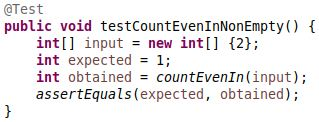
\includegraphics[width=\linewidth]{figures/stmtCoverageOrientedTests.JPG}
	\caption{Tests orientados a satisfacer cobertura de sentencias para el c\'odigo de \emph{countEvenIn(int[])} \ref{figures.code.coverageExample}.}
	\label{figures.examples.coverage.stmtTests}
\end{figure}

\begin{figure}
	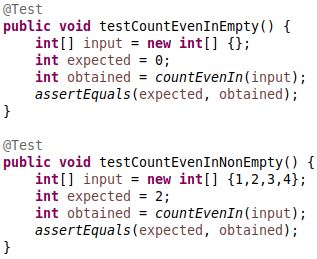
\includegraphics[width=\linewidth]{figures/branchCoverageOrientedTests.JPG}
	\caption{Tests orientados a satisfacer cobertura de ramas para el c\'odigo de \emph{countEvenIn(int[])} \ref{figures.code.coverageExample}.}
	\label{figures.examples.coverage.branchTests}
\end{figure}

\begin{figure}
	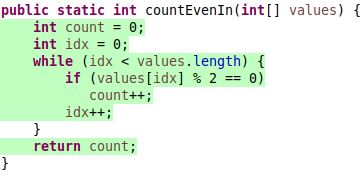
\includegraphics[width=\linewidth]{figures/branchCoverageExampleComplete.JPG}
	\caption{Medici\'on de cobertura de \emph{countEvenIn(int[])} \ref{figures.code.coverageExample} con una cobertura del 100\% tanto de sentencias como de ramas.}
	\label{figures.examples.coverage.fullCoverage}
\end{figure}

\begin{figure}
	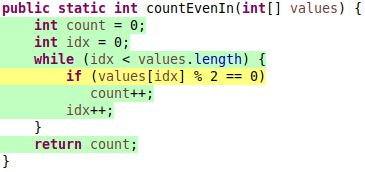
\includegraphics[width=\linewidth]{figures/branchCoverageExampleIncomplete.JPG}
	\caption{Medici\'on de cobertura de \emph{countEvenIn(int[])} \ref{figures.code.coverageExample} con una cobertura del 100\% de sentencias pero no de ramas.}
	\label{figures.examples.coverage.stmtCoverage}
\end{figure}

En el caso de criterios de caja negra, varios criterios com\'unmente utilizados se basan en analizar la especificaci\'on de las entradas esperadas por el programa a analizar. En general se comienza partiendo el dominio de cada entrada de acuerdo a ciertas caracter\'isticas provistas. \'Estas deben dividir el conjunto de valores de cada entrada en subconjuntos disjuntos, y la uni\'on de todos los subconjuntos debe resultar en el dominio completo de cada entrada. Por ejemplo, si una entrada es un entero, es posible dar como caracter\'istica a \emph{ser par}, lo que divide todo el conjunto de los enteros en dos subconjuntos disjuntos (uno conteniendo todos los enteros pares y otro conteniendo a todos los impares), tal que al unir estos conjuntos se obtiene nuevamente a todos los enteros. Cada criterio basado en las entradas del programa a evaluar define de qu\'e forma combinar valores de cada subconjunto en los casos donde el programa tiene varias entradas. Por ejemplo, combinar todos con todos, o cada subconjunto debe estar representado por lo menos una vez sin importar con qu\'e otro subconjunto es combinado. Para el ejemplo de la Figura \ref{figures.code.replaceExample}, que muestra un m\'etodo que dado un arreglo de enteros, un valor entero a buscar en el arreglo, y un valor con el cual reemplazar el valor anterior, realiza los reemplazos y retorna cuantos fueron realizados, en la Tabla \ref{tables.example.codeCoverage} se muestran posibles caracter\'isticas para dividir cada entrada: que el arreglo sea o no vac\'io; que el valor a buscar est\'e o no en el arreglo; y finalmente que el valor con el cual reemplazar al anterior sea igual o distinto al reemplazado. Vale aclarar que si bien todas las caracter\'isticas dividen las entradas en dos subconjuntos, esto no debe ser necesariamente as\'i. Una caracter\'istica que divida en m\'as subconjuntos es perfectamente v\'alida, siempre que cumpla con las propiedades mencionadas anteriormente. Como ejemplo de combinaci\'on de valores de cada subconjunto definidos por las caracter\'isticas en la Tabla \ref{tables.example.codeCoverage}, podemos utilizar el criterio \emph{Each Choice Value}, el cual determina que cada subconjunto debe estar representado al menos una vez en los tests. Esto lleva a los tests que se muestran en la Figura \ref{figures.examples.coverage.eccTests}, donde tenemos dos tests, uno donde se utiliza un arreglo no vac\'io, con el valor a reemplazar perteneciendo al arreglo (2) y el valor con el cual reemplazar siendo igual al anterior; el segundo test utiliza un arreglo vac\'io, obviamente el elemento a buscar no pertenece al mismo y el valor con el cual se realiza el reemplazo es distinto al anterior. El hecho de que como se puede apreciar en la Figura \ref{figures.examples.coverage.eccCoverage}, los tests anteriores logran una cobertura de ramas del 100\% al tiempo que \'estos son evidentemente un conjunto muy pobre de escenarios, sirve para remarcar c\'omo un criterio puede ser satisfecho al mismo tiempo que los tests que lo satisfacen son claramente de muy mala calidad.

\begin{figure}
	\lstinputlisting[basicstyle=\small, language=Java, tabsize=3]{results/draft/Replace.java}
	\caption{M\'etodo para reemplazar todos los valores en un arreglo \emph{array} que son iguales a un valor especificado (\emph{what}) por otro valor especificado (\emph{with}) y retornar cuantos cambios se realizaron.}
	\label{figures.code.replaceExample}
\end{figure}

\begin{table}[]
	\begin{tabular}{|c|ccc|}
		\hline
		Bloque & array vacío & what pertenece & with igual a what \\ \hline
		1 & T & T & T \\ \hline
		2 & F & F & F \\ \hline
	\end{tabular}
	\caption{Caracter\'isticas con las que se puede dividir los conjuntos de las entradas del programa \emph{replace(int[], int, int)} \ref{figures.code.replaceExample}.}
	\label{tables.example.codeCoverage}
\end{table}

\begin{figure}
	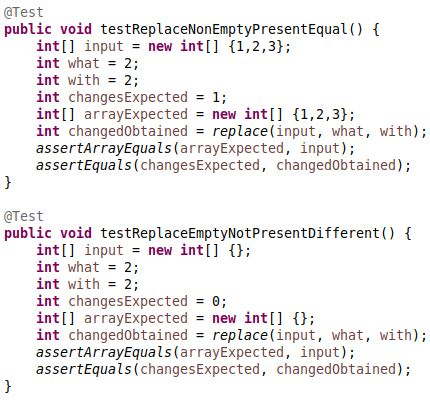
\includegraphics[width=\linewidth]{figures/replaceTestsEachChoice.JPG}
	\caption{Tests para satisfacer criterio de cobertura \emph{Each Choice Coverage} para \ref{figures.code.replaceExample} basado en las caracter\'isticas definidas en \ref{tables.example.codeCoverage}.}
	\label{figures.examples.coverage.eccTests}
\end{figure}

\begin{figure}
	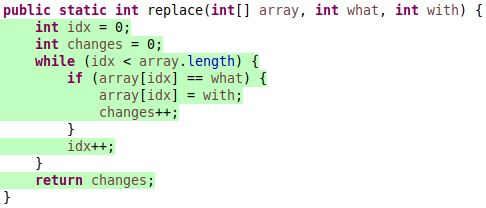
\includegraphics[width=\linewidth]{figures/replaceFullCoverage.JPG}
	\caption{Cobertura de ramas lograda por los tests definidos en \ref{figures.examples.coverage.eccTests}.}
	\label{figures.examples.coverage.eccCoverage}
\end{figure}

\chapter[Mutation]{Mutation testing}
\label{sec:preliminares.mutation}


\subsection{Evaluaci\'on de mutation testing}

Las propiedades de inter\'es en el disen\~no y evoluci\'on de operadores involucrados en mutation testing son, equivalencia de mutantes con el programa original y entre mutantes, dificultad de detecci\'on de mutantes, acoplamiento entre fallas reales y mutantes, y acoplamiento entre mutantes.

\subsubsection{Equivalencia}
Equivalencia [entre dos programas] es una propiedad definida bajo la relaci\'on \texttt{Eq(P, P$\prime$) : $\nexists$ E : P(E) != P$\prime$(E)}, la cual establece que dos programas \texttt{P} y \texttt{P$\prime$} son equivalente si no existe un escenario \texttt{E} tal que el comportamiento de ambos programas se distinto. Esta es una relaci\'on indecidible por lo que m\'etodos incompletos son utilizados. Dentro de mutation testing, equivalencia puede encontrarse entre un mutante y el programa original, un caso indeseable ya que \'estos disminuyen el valor del mutation score sin significar una deficiencia de parte del test suite en detectar ciertas fallas artificiales. Otro caso de equivalencia se da entre mutantes, un caso en donde ambos mutantes son detectados por el test suite, sin embargo al ser equivalente incrementan el valor del mutation score sin significar una mejora de parte del test suite en detectar m\'as fallas artificiales.

Dentro de la investigaci\'on sobre la detecci\'on (evaluaci\'on) de esta caracter\'istica y su impacto en el ana\'alisis de test suites usando mutation testing, \cite{biblography.mutation.evaluation.equivalent.Schuler+10} propone la utilizaci\'on de diferencia en cobertura de c\'odigo y an\'alisis de fujo de datos para determinar potencial equivalencia. Mientras que  \cite{biblography.mutation.evaluation.equivalent.Just+13} utiliza detecci\'on de restricciones condicionales para alcanzar el c\'odigo mutado y \emph{SAT Solving} para determinar si es posible satisfacer dichas restricciones al tiempo que se obtiene un valor distinto al del programa original en ese punto, lo que es similar en principio a \emph{weak mutation}, en donde se considera que un mutante es detectado si en el estado siguiente a la mutaci\'on se detecta una diferencia con el del programa original, pero a\~nadiendo control de alcanzabilidad y una verificaci\'on exhaustiva acotada para detectar si es posible que exista una diferencia.
En \cite{biblography.mutation.evaluation.equivalent.Grun+09} observan que manualmente, para los casos de estudios utilizados, un programador avanzado tarda aproximadamente 15 minutos en promedio para analizar mutantes equivalentes. Y claramente la existencia de equivalentes disminuye artificialmente el mutation score dando la falsa impresi\'on de que es necesario agregar m\'as tests.

\subsubsection{Dificultad de detecci\'on}

As\'i como los mutantes equivalentes son indeseables por ser imposibles de detectar, los mutantes que son solo detectables por un conjunto peque\~no de tests, son altamente deseables. Estos son denominados \emph{stubborn} \cite{bibliography.mutation.evaluation.stubbornHieronsHD99}. La detecci\'on de estos mutantes requieren tests de "mejor calidad" y si bien existen estudios que eval\'uan la generaci\'on de stubborns por operador \cite{bibliography.mutation.evaluation.stubborn}, \'este depende del conjunto de programas utilizados y los tests asociados. Con respecto a este obst\'aculo, en \cite{bibliography.mutation.evaluation.hardnessVisser}, proponen el uso de \emph{model counting} sobre programas m\'as simples pero utilizando un estudio m\'as exhaustivo.

\subsubsection{Subsunci\'on}

\emph{Subsumption}, la relaci\'on entre mutantes con respecto a los tests que los detectan, dan lugar a mutantes redundantes. Esto es, los tests que detectan al mutante subsumido, incluyen a aquellos que detectan al que subsume, es decir, el mutante subsumido eval\'ua de manera menos espec\'ifica a los tests ya que es detectado por una mayor cantidad, mientras que el que subsume eval\'ua tests m\'as espec\'ificos. Esto lleva a mutantes redundantes y representa una forma de evaluar la dificultad de detecci\'on, los mutantes que subsumen a otros pero no son a su vez subsumidos, son detectados por pocos tests. Presentado inicialmente en \cite{bibliography.mutation.selection.Offutt96}, mutant subsumption es utilizado por \cite{bibliography.mutation.minimizing.dynamicsubsumption} y \cite{bibliography.mutation.evaluation.JustKA17} para evaluar utilidad de mutantes dentro de mutation analysis.

\subsubsection{Acoplamiento}

\emph{Coupling}, el acoplamiento entre fallas reales y mutantes es una propiedad altamente deseable, sin la misma, mutation testing perder\'ia su utilidad al desaparecer la correlaci\'on entre un mutation score alto y una buena capacidad de parte del test suite para detectar fallas reales. El trabajo m\'as importante sobre este tema, y uno que nos representa una motivaci\'on importante para el desarrollo de nuestros operadores de mutaci\'on presentados en esta tesis, es \cite{bibliography.mutation.evaluation.valid-substitute}. El acoplamiento entre mutantes y fallas reales es una relaci\'on que especifica que si un conjunto de tests detecta un conjunto de mutantes, entonces va a detectar una falla real. 

\subsection{High order}

\texttt{High Order}, la combinaci\'on de mutaciones, generada al aplicar operadores de mutaci\'on m\'as de una vez al generar un mutante, se denominan mutaciones de alto order mientras que aquellas que la forman, se las llama de primer orden. Si bien en principio esto agregar\'ia una gran cantidad de nuevos mutantes\footnote{Usualmente la cantidad de mutantes al aplicar m\'as de una mutaci\'on por mutante est\'a acotada por M$_0^G$ en donde \texttt{M$_0$} son la cantidad de mutantes de primer orden y \texttt{G} son la cantidad de mutaciones por mutante}, los estudios actuales que se enfocan en esta t\'ecnica concluyen que estos mutantes de alto orden representan fallas artificiales m\'as sutiles y que subsumen a una gran cantidad de mutantes de primer orden. [AGREGAR]
\chapter{Mutaci\'on de expresiones de navegaci\'on en reparaci\'on de programas}
\label{cap:repair}

\section{Reparaci\'on autom\'atica de programas}
\label{sec:repair}

La aparici\'on de t\'ecnicas autom\'aticas para testing y localizaci\'on de fallas, es decir, detectar en donde puede estar una falla, una vez detectada, llev\'o a la investigaci\'on de t\'ecnicas para, una vez detectada, poder reparar dicha falla de manera autom\'atica. Pero que significa reparar una falla?
\begin{quote}
	Dado un programa \textbf{P} y una especificaci\'on \textbf{E} del mismo, si \textbf{P} no cumple con sus especificaciones (\textbf{E}), reparar al programa significa encontrar un variante \textbf{P'} mediante modificaciones sint\'acticas tal que \'esta cumpla con las especificaciones dadas por \textbf{E} \footnote{Esta definici\'on no considera reparaciones en tiempo de ejecuci\'on, es decir, aquellas que no producen una variante del programa original como reparaci\'on}.
\end{quote}
A partir del trabajo de \cite{bibliography.repair.ArcuriY08}, muchas herramientas que intentan atacar a este problema han surgido. Incluso cuando la idea de reparaci\'on autom\'atica de fallas es atractiva, reparar autom\'aticamente defectos de programas arbitrarios es inviable. Por lo tanto, la reparaci\'on autom\'atica de programas debe sacrificar completitud. Varias t\'ecnicas efectivas para reparaci\'on de programas recurren a explorar un conjunto grande (aunque limitado) de candidatos de reparaci\'on obtenidos por modificaciones sint\'acticas de un programa con fallas. Adem\'as, para que estas t\'ecnicas escalen razonzablemente, el espacio de candidatos a reparaci\'on debe ser acotado, limitando el conjunto de modificaciones sint\'acticas a considerar (por ejemplo, no considerar modificaciones a partes de una sentencia), o no explorando exhaustivamente el conjunto acotado de candidatos a reparaci\'on (por ejemplo, usando algor\'itmos gen\'eticos en lugar de b\'usqueda exhaustiva).

\subsection{Or\'aculo de reparaci\'on}
\label{sec:repair.specs}

En general el proceso de reparaci\'on sigue, a rasgos muy generales, el siguiente algoritmo:

\begin{lstlisting}[basicstyle={}, language=Java]
  repair(P, E) {
    current = P
    while (!isValid(current, E) && !boundsReached()) {
      current = nextFix();
    }
    return current;
  }
\end{lstlisting}

Donde \textbf{P} representa el programa a reparar, y \textbf{E} las especificaciones que se deben satisfacer. El proceso b\'usca candidatos a reparaciones, evaluando a \'estos con respecto a las especificaciones provistas. Claramente el proceso est\'a acotado a un conjunto finito de posibles reparaciones.

Evidentemente, es necesario definir que se usa como especificaciones para el programa. Los primeros trabajos sobre reparaci\'on autom\'atica \cite{bibliography.repair.StaberJB05, bibliography.repair.ArcuriY08}, utilizaban especificaciones formales en forma de pre y post condiciones, o descripciones l\'ogicas provistas en alg\'un formalismo l\'ogico apropiado. Sin embargo, muchas de las \'ultimas t\'ecnicas utilizan tests como especificaciones. La raz\'on principal detr\'as de esto, es el argumento de que la producci\'on de especificaciones formales es un proceso costoso, a la vez que es muy raro encontrarlas ya provistas previo al proceso de reparaci\'on, mientras que los tests son menos costosos de proveer y es mucho m\'as com\'un encontrarlos ya provistos antes del proceso de reparaci\'on.

Por ejemplo, \emph{GenProg} \cite{bibliography.repair.GouesNFW12} usa computaci\'on evolutiva para evolucionar sint\'acticamente un programa hasta que una reparaci\'on aceptable es encontrada. Cada reparaci\'on candidata (modificaci\'on sint\'actica) es aplicada al programa original para producir uno nuevo cuya aptitud es evaluada utilizando un test suite. Modificaciones sint\'acticas en partes de una sentencia no son consideradas para limitar el espacio de candidatos, y la funci\'on de aptitud es utilizada para mantener una poblaci\'on reducida de candidatos a lo largo del proceso de computaci\'on evolutiva. 

\subsubsection{Tests como especificaciones}
\label{sec:repair.specs.testsAsSpecs}

Las herramientas actuales, en general, utilizan tests como especificaciones parciales del programa a reparar. Esto tiene como consecuencia la generaci\'on de reparaciones espurias, es decir, reparaciones que si bien logran hacer ``pasar'' a los tests, no resuelven el problema. En muchos casos, enmascarar un defecto puede causar que los tests que antes detectaban una falla, ahora dejen de hacerlo. A modo de ejemplo, en la Figura~\ref{figures.examples.repair.nullaccessexample} se muestra un m\'etodo \emph{find(int)} que tiene un defecto, la condici\'on del \textbf{while} deber\'ia incluir que \textbf{current} no sea \emph{null} y que el elemento a\'un no fue encontrado. Sin embargo, la reparaci\'on en la Figura~\ref{figures.examples.repair.nullaccessexample.mask} enmascara al defecto. Si nuestros tests solo utilizan listas en donde el elemento no est\'a, y por lo tanto se espera que el m\'etodo retorne \emph{false}; o el elemento a buscar est\'a en la \'ultima posici\'on, y se espera que retorne \emph{true}. La reparaci\'on anterior es espuria, es decir, si bien logra que los tests terminen correctamente, no repara realmente el programa.

\begin{figure}
	\begin{lstlisting}[frame=single, mathescape=true,language=Java,basicstyle={},framexleftmargin=.073\textwidth,xleftmargin=.085\textwidth,xrightmargin=0.012\textwidth]
  public boolean find(int e) {
    if (isEmpty()) return false;
    Node current = header;
    boolean found = false;
    while(true) {
      found = current.elem == e;
      current = current.next;
    }
    return found;
  }
	\end{lstlisting}
	\caption[Ejemplo de bug causando \emph{NullPointerException}]{Un m\'etodo con un defecto que causa \emph{NullPointerException}}
	\label{figures.examples.repair.nullaccessexample}
\end{figure}

\begin{figure}
	\begin{lstlisting}[frame=single, mathescape=true,language=Java,basicstyle={},framexleftmargin=.073\textwidth,xleftmargin=.085\textwidth,xrightmargin=0.012\textwidth]
  public boolean find(int e) {
    if (isEmpty()) return false;
    Node current = header;
    boolean found = false;
    while(true) {
      try {
        found = current.elem == e;
        current = current.next;
      } catch (NullPointerException e) {
        break;
      }
    }
    return found;
  }
	\end{lstlisting}
	\caption{Reparaci\'on que enmascara el defecto en la Figura~\ref{figures.examples.repair.nullaccessexample}}
	\label{figures.examples.repair.nullaccessexample.mask}
\end{figure}

Esta observaci\'on llev\'o a un trabajo de investigaci\'on en donde se evaluaron un conjunto de herramientas actuales de reparaci\'on autom\'atica de programas basadas en tests como or\'aculo de reparaci\'on \cite{bibliography.repair.ZeminBGCDRAF17}. Al contrario de trabajos previos que se basaron en tests o inspecci\'on manual de las reparaciones provistas por las herramientas evaluadas (\emph{GenProg}, \emph{Angelix}, \emph{AutoFix}, y \emph{Nopol}, entre otras), en \'este, se utilizaron especificaciones formales y \emph{PEX} \cite{bibliography.formalver.TillmannH08} para evaluar las reparaciones obtenidas.

Los resultados obtenidos, logrados sobre el benchmark de reparaci\'on de programas \emph{IntroClass} \cite{bibliography.repair.benchmarks.GouesHSBDFW15}, indican que al evaluar las reparaciones producidas utilizando especificaciones formales, \'estas son inv\'alidas, es decir, el programa obtenido no cumple con las especificaciones del problema que deben resolver. El porcentaje de reparaciones para \emph{GenProg}, que son consideradas como efectivas, es solo un 1.57\% (18 de 1.143 fallas fueron reparadas) de las cuales 8 reparan errores de typos en cadenas asociadas a los mensajes de salida del programa. \emph{Angelix} solo es capaz de reparar 41 de 232 (17,67\%), \emph{Nopol} solo 6 de 297 (2\%), y finalmente \emph{AutoFix} no pudo reparar ning\'un programa de manera correcta\footnote{Algunas herramientas no soportaban ciertas caracter\'isticas (retornar una cadena), y en otras que requer\'ian traducir a otro lenguaje, la misma reparaba el defecto}. Por el otro lado, incrementar la cantidad de tests disminu\'ia dr\'asticamente las reparaciones espurias, pero tambi\'en las reparaciones en general. En otros casos, las herramientas no soportaban el aumento en la cantidad de tests.

\subsection{Granularidad de las reparaciones}
\label{sec:repair.granularity}

Como mencionamos anteriormente, el conjunto de candidatos a reparaci\'on a tener en cuenta, debe ser finito y su tama\~no afecta directamente a los recursos necesarios para reparar el programa. Esto genera una necesidad de balancear capacidad de reparaci\'on, es decir, que tipo de fallas se pueden reparar, con recursos necesarios. Por ejemplo, el caso de \emph{GenProg}, se basa en mover, duplicar, o eliminar c\'odigo. La idea es que muchas veces un desarrollador escribe varias veces el mismo c\'odigo, por ejemplo, sumarle 1 a una variable. Por otro lado, en \emph{SPR} \cite{bibliography.repair.LongR15}, se generan reparaci\'ones abstractas como agregar una condici\'on \textbf{C} antes de la ejecuci\'on de una sentencia, la cual luego ser\'a reemplazada por una condici\'on concreta en una etapa posterior, esto sumado a la eliminaci\'on, y duplicaci\'on de c\'odigo existente. En \emph{PAR} \cite{bibliography.repair.KimNSK13}, las modificaciones para reparar el programa son aprendidas a partir de patrones en reparaciones escritas manualmente. Por esto, el n\'umero de candidatos a considerar como reparaciones es significativamente reducido, lo que a su vez reduce el tipo de errores que la t\'ecnica puede ser capaz de reparar.

Modificaciones a partes de sentencias, es decir, aquellas que alteran expresiones dentro de una sentencia, son en general no consideradas por t\'ecnicas de reparaci\'on de programas. Una limitaci\'on principal al considerar a \'estas, es la explosi\'on en el espacio de candidatos de reparaci\'on. T\'ecnicas que utilizan operadores de mutaci\'on para producir las modificaciones sint\'acticas, y que incluyen modificaciones a partes de sentencias, requieren limitar el conjunto de mutaciones (por ejemplo, \cite{bibliography.repair.GopinathMK11}), reduciendo la clase de fallas que \'estas pueden intentar reparar.

\begin{figure}
\footnotesize
\begin{lstlisting}[frame=single, mathescape=true,language=Java,basicstyle={},xleftmargin=.010\textwidth,xrightmargin=.007\textwidth]
boolean add(Object arg) {
  SListNode freshNode = new SListNode();
  freshNode.value = arg;
  boolean added = false;
  if (this.header == null) {
    this.header = freshNode;
    added = true;
  } else {
    SListNode current = this.header.next; //BUG: ignora primer nodo
    while (current.next ! = null && current.value ! = arg) {
      current = current.next;
    }
    if (current.value ! = arg) {
      current.next = freshNode;
      added = true;
    }
  }
  if (added) {
    size = size - 1; //BUG: decrementa size
  }
  return added;
}
\end{lstlisting}
\caption[Programa con dos bugs intra-sentencia]{Ejemplo de c\'odigo con dos bugs que requieren modificaciones intra-sentencia}
\label{figures.examples.repair.exampleCode}
\end{figure}

Los efectos que tienen estas restricciones sobre el espacio de candidatos a considerar para la reparaci\'on, pueden observarse en la Figura~\ref{figures.examples.repair.exampleCode} donde se muestra el m\'etodo \emph{add(Object)} de un conjunto. \'Este contiene dos defectos: primero, cuando el conjunto no est\'a vaci\'o, se comienza el recorrido del mismo a partir del nodo siguiente al inicial (el cual podr\'ia ser \emph{null}, resultando en un error en la l\'inea siguiente); segundo, cuando un nuevo nodo es agregado a la lista sobre la cual est\'a implementado el conjunto, el tama\~no de la misma (atributo \emph{size}) se decrementa. Para reparar al m\'etodo es necesario realizar dos cambios, ambos dentro de una sentencia. En herramientas que hacen cambios a nivel bloque, solo es posible reparar el programa si existen en otro punto del c\'odigo las sentencias \textbf{current = this.header;} y \textbf{size = size + 1}.


\subsubsection{Mutaci\'on en reparaci\'on}
\label{sec:repair.granularity.mutation}

El uso de operadores de mutaci\'on, provenientes de mutation testing, en reparaci\'on de programas, parece razonable: si estos operadores son utilizados en mutation testing para emular defectos reales, podr\'ian utilizarse para emular reparaciones. Ejemplos recientes de herramientas de reparaci\'on autom\'atica de programas son \cite{bibliography.repair.mutation.DebroyW10} y  \cite{bibliography.repair.mutation.AlloyWang18}. El argumento de utilizar mutaci\'on en reparaci\'on de programas es que existen mutaciones que si se fueran a combinar, se cancelar\'ian, por ejemplo:
\begin{lstlisting}[mathescape=true, language=Java,basicstyle={}]
  for (int i = 0; i < lenght; i++)...
  $\Delta$for (int i = 0; i > lenght; i++)...
\end{lstlisting}
donde la primera sentencia se puede mutar, aplicando un cambio de operador relacional, a la segunda, marcada por $\Delta$, que a su vez se puede mutar al c\'odigo original aplicando el mismo operador de mutaci\'on. Aunque no siempre se puede deshacer una mutaci\'on aplicando otra que sea sint\'acticamente inversa. 
Volviendo al ejemplo anterior, el mutante:
\begin{lstlisting}[mathescape=true, language=Java,basicstyle={}]
  for (int i = 0; i > lenght; i++)...
\end{lstlisting}
puede ser restaurado, sem\'anticamente, generando el mutante:
\begin{lstlisting}[mathescape=true, language=Java,basicstyle={}]
  for (int i = 0; i $\textbf{!=}$ lenght; i++)...
\end{lstlisting}
Existen tambi\'en casos donde varias mutaciones pueden corregir el comportamiento. Esto lleva a la idea de que si consideramos el programa con fallas \texttt{P$_b$} y el original sin fallas \texttt{P$_o$}, se puede definir el segundo en t\'erminos del primero como \texttt{P$_b$ = mutate(P$_o$, M)} donde \texttt{M} representa una secuencia de mutaciones y \texttt{mutate} es un programa que aplica dicha secuencia a un programa. En general como dijimos anteriormente, muchas mutaciones tienen su inversa, ya sea sint\'actica o sem\'antica, lo que lleva a definir el problema de reparaci\'on como encontrar una secuencia de mutaciones \texttt{M$\prime$} tal que \texttt{P$_o$ = mutate(P$_b$, M$\prime$)}.

La reparaci\'on de programas puede describirse como una b\'usqueda exhaustiva que, dado un programa defectuoso y una especificaci\'on del mismo (que como vimos puede ser formal o mediante tests), y un conjunto de operadores de mutaci\'on:
\begin{enumerate}
	\item Considera el programa a reparar como el candidato a reparaci\'on inicial.
	
	\item Si \textbf{P} es un candidato a reparaci\'on, y \textbf{Q} es el resultado de aplicar una mutaci\'on a \textbf{P}, entonces \textbf{Q} tambi\'en es un candidato a reparaci\'on.
	
	\item  Un candidato \textbf{S} es exitoso si satisface las especificaciones provistas.
\end{enumerate}

\begin{figure}
	\centering
	\begin{tikzpicture}%
	[state/.style ={ellipse, draw, minimum width = 0.7 cm},
	point/.style = {circle, draw, inner sep=0.04cm,fill,node contents={}},
	el/.style = {inner sep=2pt, align=left, sloped}]
	\node[state,rectangle] (init) {$return\:a < b?a:b;$};
	\node[state,rectangle] (cand1) [below=of init] {$return\:b < b?a:b;$};
	\node[state,rectangle] (cand2) [right=of cand1] {$return\:a < b?a:0;$};
	\node[state,rectangle] (succ) [below=of cand1] {$return\:b < a?a:b;$};
	
	\path[->] (init) edge node[left] {a -> b} (cand1);
	\path[->] (init) edge node[right=16pt] {b -> 0} (cand2);
	\path[->] (cand1) edge node[left] {b -> a} (succ);
	
	\node[label=right: {\small Inicial}, draw=blue,dotted,fit=(init)] (initR) {};
	
	\node[label=right: {\small Candidatos (Profundidad 1)},draw=blue,dotted,fit=(cand1) (cand2), inner sep=0.2cm] (Candidates) {};
	
	\node[label=right: {\small Exitoso (Profundidad 2)},draw=blue,dotted,fit=(succ)] (Succ) {};
	
	\end{tikzpicture}
	\caption[Reparaci\'on como b\'usqueda, ejemplo]{Reparaci\'on de un programa que calcula el m\'aximo de dos n\'umeros}
	\label{figures.examples.repairWithMutation}
\end{figure}

La definici\'on previa de reparaci\'on autom\'atica de programas deja en claro que el espacio de candidatos a reparaci\'on depende del n\'umero de mutaciones (\textbf{b}) a considerar, lo que influye en cuan ``ancho'' es el \'arbol de b\'usqueda, y el n\'umero m\'aximo de mutaciones sucesivas permitidas (\textbf{d}) para generar a los candidatos, lo que afecta la profundidad de la b\'usqueda. El espacio de b\'usqueda queda entonces definido por una suma geom\'etrica $\frac{b^{d+1}-1}{b-1}$ ($O(b^d)$). Si consideramos el m\'etodo en la Figura~\ref{figures.examples.repair.getNode}, y solo cuatro l\'ineas del mismo, al utilizar 18 operadores de mutaci\'on (mediante la herramienta \emph{$\mu$Java++}), podemos ver en la Tabla \ref{tables.repair.mutation.explosion}, como a medida que aumentamos la cantidad de mutaciones consecutivas (la profundidad en reparaci\'on mediante mutaci\'on), la cantidad de candidatos a evaluar se vuelve r\'apidamente inmanejable.

\begin{figure}
	\begin{lstlisting}[frame=single, mathescape=true,language=Java,basicstyle={},framexleftmargin=.073\textwidth,xleftmargin=.085\textwidth,xrightmargin=0.012\textwidth]
  Node getNode(int i) {
    Node current = this.head;
    Node result = null;
    int current_index = 0;
    while (result == null && current != null) {
      if (i == current_index ) {
        result = current;
      }
      current_index = current_index + 1;
      current = current.next;
    }
    return result;
  }
	\end{lstlisting}
	\caption[M\'etodo de ejemplo, \emph{getNode(int)}]{C\'odigo de ejemplo, m\'etodo que obtiene el i-\'esimo nodo de una lista}
	\label{figures.examples.repair.getNode}
\end{figure}

\begin{table}[t]
	\caption[Mutantes para \emph{getNode} (Figura~\ref{figures.examples.repair.getNode}) a diferentes profundidades]{Mutantes generados para \emph{getNode} de la Figura~\ref{figures.examples.repair.getNode}, considerando 4 l\'ineas y 18 operadores, a medida que la profundidad aumenta.}
	\label{tables.repair.mutation.explosion}
	\begin{center}
		\small
		\begin{tabular}{c r}
			Search Depth                            &	No. of Mutants (Fix Candidates)        \\
			\hline
			1 					&	40		                               	\\
			2 					&	1,604			                \\
			3 					&	64,684		        	        \\
			4 					&	$>$ 20 million		                
		\end{tabular}
		\normalsize
	\end{center}
\end{table}

\pagebreak
\subsection{Striker}
\label{sec:repair.striker}

\emph{Striker} es una herramienta de reparaci\'on autom\'atica de programas cuya meta principal es:
\begin{quote}
	Proveer una t\'ecnica automatizada y eficiente para reparar programas anotados con especificaciones (en t\'erminos de pre y post condiciones) corrigiendo errores que resultan como una consecuencia de ocurrencias simultaneas de un n\'umero de errores sint\'acticos dentro de sentencias de un programa.
\end{quote}
Es necesario remarcar la necesidad de especificaciones asociadas al programa. As\'i tambi\'en, los errores que se consideran son defectos, o mutaciones, dentro de sentencias. En particular no se apunta a reparar programas que requieran agregar, o eliminar, c\'odigo. Algunos de los defectos reparables por \emph{Striker} se muestran en la Figura~\ref{figures.examples.repair.faultsGetNode}.

Si bien muchas herramientas de reparaci\'on autom\'atica de programas utilizan mutaci\'on, \emph{Striker} es una de las m\'as flexibles con respecto a operadores soportados, entre ellos \emph{PRVO}; soporte para modificaciones a partes de sentencias; y fallas que requieren las modificaci\'on de varias sentencias. Striker utiliza \emph{TACO} \cite{bibliography.mutation.tools.TACOGaleottiRPF13} para evaluar candidatos a reparaci\'on, lo que requiere proveer especificaciones formales en lugar de un test suite, y JML RAC \cite{bibliography.misc.JMLRAC.LeavensCCRC02} como t\'ecnica de evaluaci\'on r\'apida basada en escenarios previamente encontrados para los cuales un candidato a reparaci\'on no cumpl\'ia con las especificaciones. Sin entrar en detalles, esta herramienta es capaz de expandir las fallas soportadas para reparar, agregando varios operadores en los que se incluye a \emph{PRVO}, y permitir la reparaci\'on de aquellas que requieren modificaciones intra-sentencias as\'i como en m\'ultiples sentencias, mediante el uso de t\'ecnicas de poda innovadoras.

Bajo esta herramienta es que se pudo observar como \emph{PRVO} era capaz de reparar ciertas fallas que de otra forma no eran reparables, como por ejemplo el caso de \emph{add(int)} en la Figura~\ref{figures.examples.repair.exampleCode}, en donde si bien el segundo defecto es reparable por \emph{AORB} el cual reemplaza el operador incorrecto (\emph{-}) por el que corresponde (\emph{+}), el primer defecto solo puede ser reparado por \emph{PRVO} al eliminar el acceso al campo \emph{next}. Si bien el enfoque principal de esta tesis se encuentra en \emph{PRVO} como un operador de mutaci\'on en el contexto de mutation testing, es interesante mostrar su contribuci\'on en el contexto de reparaci\'on.

\begin{figure}[t]
	\footnotesize
	$$
	\begin{array}{rl}
	5_a: & (\mathit{result} \mbox{ != }\mathsf{null}\ \&\&\ \mathit{current}\mbox{ != }\mathsf{null})\\
	5_b: & (\mathit{result} == \mathsf{null}\ \&\&\ \mathit{current} == \mathsf{null})\\
	5_c: & (\mathit{result} == \mathsf{null}\ ||\ \mathit{current}\mbox{ != }\mathsf{null})\\
	6_a: & (\mathit{i} == \mathit{current\_index} + 1)\\
	6_b: & (\mathit{i}\ \mbox{!=}\ \mathit{current\_index})\\
	9_a: & \mathit{current\_index} = \mathit{current\_index} - 1\\
	10_a: & \mathit{current.next} = \mathit{current}
	\end{array}
	$$
	\normalsize
	\caption[Defectos del algoritmo en la Figura~\ref{figures.examples.repair.getNode} reparables por \emph{PRVO}]{Algunos defectos en el m\'etodo \emph{getNode} de la Figura~\ref{figures.examples.repair.getNode} que pueden modelarse mediante mutaciones y ser reparados por \emph{PRVO}.}
	\label{figures.examples.repair.faultsGetNode}
\end{figure}

\subsection{Evaluaci\'on de Stryker}
\label{sec:repair.striker.evaluation}

Si bien la evaluaci\'on de \emph{Stryker} se encuentra enfocada hacia la t\'ecnica de poda del espacio de b\'usqueda de candidatos a reparaci\'on, lo que a su vez permite la utilizaci\'on de una mayor cantidad de operadores de mutaci\'on orientados hacia la reparaci\'on de fallas intra-sentencia, en el contexto de esta tesis nos interesan los resultados asociados a \emph{PRVO} y su utilidad en el campo de reparaci\'on autom\'atica de programas mediante operadores de mutaci\'on utilizados en mutation testing, los cuales son m\'as granulares en el tipo de cambios que realizan lo que permite incrementar la reparabilidad de programas.

En los experimentos realizados para la evaluaci\'on de \emph{Stryker}, se utilizaron implementaciones en \emph{Java} de estructuras que representan colecciones. Estas clases, para las cuales se definieron especificaciones en forma de contratos \emph{JML}, incluyendo clausulas \texttt{requires/ensures}, funciones de variantes de ciclos e invariantes de clases, son las siguientes:
\begin{itemize}
	\item \textbf{SinglyLinkedList :} Una implementaci\'on de listas simplemente encadenadas. Donde consideramos un m\'etodo \emph{contains} para evaluar pertenencia, \emph{getNode} para obtener el i-\'esimo elemento en la lista, y el m\'etodo \emph{insert} para agregar un nuevo elemento a la lista.
	
	\item \textbf{NodeCachingLinkedList :} Una lista circular, doblemente encadenada y con una cache de nodos. Considerando los m\'etodos \emph{contains}, \emph{inserte}, y \emph{remove}. Siendo el \'ultimo de particular inter\'es por almacenar nodos removidos en la cache.
	
	\item \textbf{BinarySearchTree :} Una implementaci\'on de un \'arbol de b\'usqueda binario con los m\'etodos \emph{contains}, \emph{insert} y \emph{remove}.
	
	\item \textbf{BinomialHeap :} Una implementaci\'on de colas de prioridad utilizando \emph{binomial heaps}. Considerando los m\'etodos \emph{findMin} (para obtener el m\'inimo elemento almacenado), \emph{insert}, y \emph{extractMin} para obtener y eliminar el m\'inimo elemento almacenado.
\end{itemize}

Los casos de estudio para reparaci\'on fueron obtenidos a partir de las versiones originales (correctamente implementadas) al insertar hasta $4$ mutaciones por m\'etodo, y luego se eligieron 5 versiones al azar por cada n\'umero de mutaciones insertadas, es decir, 5 programas incorrectos con un bug, 5 con 2, y as\'i hasta $4$ bugs.

Por cada sentencia (o l\'inea) mutada se agrego un comentario de l\'inea \texttt{//mutGenLimit K} donde \texttt{K} corresponde a la cantidad de bugs artificiales introducidos en la misma. Algunos ejemplos de los casos de estudios utilizados se muestran a continuaci\'on.

\begin{figure}[H]
	\lstinputlisting[basicstyle=\footnotesize, language=Java, tabsize=1,literate={\ \ }{{\ }}1]{results/repair/BinomialHeap_extractMin_orig.java}
	\caption[\emph{BinomialHeap\#extractMin}, original con contratos]{Versi\'on original del m\'etodo \emph{extractMin} de \emph{BinomialHeap} con los contratos asociados al m\'etodo.}
	\label{figures.code.repair.binheap_extractMin_orig}
\end{figure}

\begin{figure}[H]
	\lstinputlisting[basicstyle=\footnotesize, language=Java, tabsize=1,literate={\ \ }{{\ }}1]{results/repair/BinomialHeap_extractMin_4bugs.java}
	\caption[\emph{BinomialHeap\#extractMin}, $4$ bugs]{Versi\'on con $4$ bugs artificiales del m\'etodo \emph{extractMin} de \emph{BinomialHeap}.}
	\label{figures.code.repair.binheap_extractMin_4bugs}
\end{figure}

\begin{figure}[H]
	\lstinputlisting[basicstyle=\footnotesize, language=Java, tabsize=1,literate={\ \ }{{\ }}1]{results/repair/BinTree_insert_orig.java}
	\caption[\emph{BinarySearchTree\#insert}, original con contratos]{Versi\'on original del m\'etodo \emph{insert} de \emph{BinarySearchTree} con los contratos asociados al m\'etodo.}
	\label{figures.code.repair.bintree_insert_orig}
\end{figure}

\begin{figure}[H]
	\lstinputlisting[basicstyle=\footnotesize, language=Java, tabsize=1,literate={\ \ }{{\ }}1]{results/repair/BinTree_insert_3bugs.java}
	\caption[\emph{BinarySearchTree\#insert}, $3$ bugs]{Versi\'on con $3$ bugs artificiales del m\'etodo \emph{insert} de \emph{BinarySearchTree}.}
	\label{figures.code.repair.bintree_insert_3bugs}
\end{figure}

\begin{figure}[H]
	\lstinputlisting[basicstyle=\footnotesize, language=Java, tabsize=1,literate={\ \ }{{\ }}1]{results/repair/NCLL_contains_orig.java}
	\caption[\emph{NodeCachingLinkedList\#contains}, original con contratos]{Versi\'on original del m\'etodo \emph{contains} de \emph{NodeCachingLinkedList} con los contratos asociados al m\'etodo.}
	\label{figures.code.repair.ncll_contains_orig}
\end{figure}

\begin{figure}[H]
	\lstinputlisting[basicstyle=\footnotesize, language=Java, tabsize=1,literate={\ \ }{{\ }}1]{results/repair/NCLL_contains_4bugs.java}
	\caption[\emph{NodeCachingLinkedList\#contains}, $4$ bugs]{Versi\'on con $4$ bugs artificiales del m\'etodo \emph{contains} de \emph{NodeCachingLinkedList}.}
	\label{figures.code.repair.ncll_contains_4bugs}
\end{figure}

Cuando las sentencias marcadas para reparar (anotaci\'on \texttt{//mutGenLimit K}) resultaron ser un superconjunto de las sentencias con defectos, \emph{Stryker} fue capaz de reparar hasta $4$ bugs. En caso contrario \emph{Stryker} fue capaz de limitar considerablemente el espacio de b\'usqueda explorado.

%\include{requisitos-software}

%\part{Elaboraci\'on Formal de Requisitos de Software} %\ctparttext{text}
%\cleardoublepage\null
%\include{kaos-analisis}

%\part{Validaci\'on y Verificaci\'on de Requisitos de Software} %\ctparttext{text}
%\cleardoublepage\null
%\include{scr-analisis}

%\part{Conclusiones}
%\cleardoublepage
%%!TEX root = rdegiovanni-phd-tesis.tex
\chapter{Conclusiones y Trabajos Futuros}
\label{cap:conclusion}
En las \'ultimas d\'ecadas los m\'etodos formales han ganado una influencia notable dentro de la Ingenier\'ia de Requisitos. Tal es el caso de las metodolog\'ias orientadas a objetivos y las notaciones tabulares, que han logrado gran aceptaci\'on y se han aplicado sobre numerosos casos pr\'acticos.
El uso de lenguajes formales permite, entre otras cosas, eliminar todo tipo de ambig\"uedades sobre las especificaciones de requisitos, y las hace adecuadas para el an\'alisis autom\'atico, por ejemplo, para el chequeo de consistencia y completitud de los requisitos. Sin embargo, otras \'areas de la Ingenier\'ia de Software, como la verificaci\'on autom\'atica de programas, han sabido explotar en mayor medida el poder de los mecanismos de an\'alisis asociados a los m\'etodos formales, como SAT Solving e interpolaci\'on. 

En esta tesis, mostramos que es posible aprovechar este poder de an\'alisis que proveen los m\'etodos formales a lo largo de todo el proceso de ingenier\'ia de requisitos, contribuyendo a la elaboraci\'on y construcci\'on de requisitos de software (etapa temprana del proceso de requisitos), y a la validaci\'on y verificaci\'on de las especificaciones de requisitos construidas (etapa tard\'ia del proceso de requisitos). 
Mostramos adem\'as, que nuestras t\'ecnicas no s\'olo logran mejores niveles de escalabilidad que las t\'ecnicas relacionadas en el estado del arte del \'area, sino que adem\'as pueden aplicarse a casos m\'as generales (como es el caso de nuestra t\'ecnica de operacionalizaci\'on de objetivos, que puede lidiar con un amplio conjunto de propiedades de liveness).
%Sin embargo, los m\'etodos formales tienen poderosos mecanismos de an\'alisis asociados, como SAT Solving e interpolaci\'on, que han sabido ser explotados en gran medida en otras areas de la Ingenier\'ia de Software, como la verificaci\'on autom\'atica de programas. 
%A nuestro criterio, \'este poder de an\'alisis que proveen los m\'etodos formales puede ser aprovechado para asistir al ingeniero en tareas relacionadas a la elaboraci\'on y construcci\'on de requisitos de software, y no s\'olo la autom\'atizaci\'on de ciertos an\'alisis.
%En esta tesis, hemos mostrado que \'este poder de an\'alisis que proveen los m\'etodos formales, puede ser aprovechado para asistir al ingeniero en tareas relacionadas a la elaboraci\'on y construcci\'on de requisitos de software, y no s\'olo la autom\'atizaci\'on de ciertos an\'alisis.


\section{Conclusiones}
La principal contribuci\'on de esta tesis es el desarrollo de dos novedosas t\'ecnicas \emph{autom\'aticas} que, mediante la manipulaci\'on l\'ogica de f\'ormulas, asisten al ingeniero en tareas espec\'ificas llevadas a cabo a lo largo del proceso de ingenier\'ia de requisitos. 
Nuestra primera t\'ecnica ayuda al ingeniero a resolver la incompletitud de los requisitos operacionales, garantizando que la especificaci\'on obtenida satisface un conjunto de propiedades deseables. 
Por otro lado, la segunda t\'ecnica nos permite analizar si el comportamiento descripto por nuestras especificaciones de requisitos cumplen con las expectativas del cliente (validaci\'on) y se corresponde con la implementaci\'on del sistema (verificaci\'on).
Puede notarse que, en general, nuestra primera t\'ecnica es m\'as aplicable durante la etapa temprana del proceso de ingenier\'ia de requisitos, donde el ingeniero debe lidiar y resolver la parcialidad de los requisitos; mientras que la segunta t\'ecnica, requiere una descripci\'on m\'as precisa y acabada de los requisitos, por lo que es aplicable en la etapa tard\'ia de la ingenier\'ia de requisitos.


En el \cref{cap:KAOS-analisis} presentamos una t\'ecnica para la \emph{operacionalizaci\'on autom\'atica de objetivos}. B\'asicamente, nuestra t\'ecnica utiliza model checking para detectar la incompletitud de un Modelo Operacional respecto a un conjunto de objetivos, y de manera autom\'atica, combinando interpolaci\'on y SAT solving, refina las condiciones requeridas necesarias para garantizar la satisfacci\'on de los objetivos. Esta t\'ecnica propone dos contribuciones destacadas.
Primero, nuestro enfoque es completamente autom\'atico, a diferencia de los existentes que son manuales \cite{LetierVanLamsweerde2002} o a lo sumo semi-autom\'aticos \cite{Alrajeh+2009}, requiriendo la asistencia del usuario en el proceso de refinamiento. Segundo, nuestra t\'ecnica es capaz de lidiar con un amplio rango de propiedades de \emph{liveness}, mientras que los enfoque previos para la operacionalizaci\'on de objetivos \cite{LetierVanLamsweerde2002,Alrajeh+2009} s\'olo aplican a objetivos de safety y a un tipo muy particular de propiedades de progreso, que es el progreso del tiempo (\textit{Time Progress}).
Adem\'as demostramos que nuestra t\'ecnica es correcta y garantiza terminaci\'on cuando tratamos con objetivos de safety. M\'as a\'un, brindamos una metodolog\'ia que el ingeniero de requisitos puede seguir, para acercarse lo m\'as posible a la soluci\'on \'optima, en la \cref{sec:KAOS.metodologia}.

En el \cref{cap:SCR-analisis} presentamos una t\'ecnica autom\'atica para el an\'alisis de especificaciones de requisitos, aplicada a tareas ligadas a la \emph{validaci\'on} y \emph{verificaci\'on} de requisitos.
En particular, mostramos que nuestra t\'ecnica puede ser utilizada para generar casos de tests y verificar propiedades sobre las especificaciones de requisitos. 
B\'asicamente, la t\'ecnica aplica un proceso de \emph{abstracci\'on autom\'atico}, demostrado ser correcto, logrando notables mejoras en la eficiencia y escalabilidad respecto a las t\'ecnicas existentes. La principal contribuci\'on de esta t\'ecnica es que puede lidiar con el nivel de detalle original de las especificaciones, sin someterlas a reducciones manuales o fallar en el proceso de an\'alisis cuando otras t\'ecnicas lo hacen. Esto permite, entre otras cosas, que los casos de tests generados (o las violaciones detectadas) puedan ser directamente contrastados con las expectativas del usuario (validaci\'on) y con el comportamiento real del sistema implementado (verificaci\'on). 

%Todos los casos de estudio presentados en esta tesis, pueden descargarse desde {\small\url{http://dc.exa.unrc.edu.ar/staff/rdegiovanni/es/casos-de-estudio.html}} y reproducirse siguiendo las instrucciones que all\'i se pueden encontrar.

%Es importante mencionar, que las t\'ecnicas presentadas en esta tesis est\'an basadas y extienden art\'iculos que hemos publicado recientemente \cite{Degiovanni+2011,Degiovanni+2014}. 
%Adem\'as, en colaboraci\'on con otros investigadores, y gracias a lo aprendido en este trabajo, hemos publicado \cite{Scilingo+2013,Scilingo+2014,Regis+2015}.


\section{Trabajos Futuros}

Tenemos varias l\'ineas de trabajos futuros. 
Por un lado, planeamos aplicar nuestra t\'ecnica de operacionalizaci\'on de objetivos sobre casos de estudio m\'as grandes, que nos permitan evaluar si existen problemas de escalabilidad, para as\'i realizar las mejoras necesarias. Adem\'as, planeamos investigar cu\'al es la relaci\'on precisa entre las operacionalizaciones obtenidas por interpolaci\'on con aquellas obtenidas con programaci\'on l\'ogica inductiva (ILP). En particular, estamos interesados en analizar una posible noci\'on de operacionalizaci\'on ``m\'as general'', y evaluar si el refinamiento basado en interpolaci\'on nos permite alcanzar dicha operacionalizaci\'on.  Adem\'as, planeamos investigar una potencial complementaci\'on entre interpolaci\'on e ILP, para la operacionalizaci\'on de objetivos. 

Por otro lado, estamos estudiando la posibilidad de utilizar interpolaci\'on para la detecci\'on y resoluci\'on de conflictos a nivel de objetivos. Intuitivamente, podemos pensar a un interpolante sobre dos objetivos inconsistentes, como un obst\'aculo, es decir, una condici\'on cuya validez garantiza que no podr\'an ser satisfechos ambos objetivos a la vez.

Finalmente, debido a que nuestras t\'ecnicas recaen fuertemente en el c\'omputo de interpolantes, planeamos evaluar mecanismos alternativos que computan interpolantes, para analizar si alg\'un algoritmo particular de interpolaci\'on es m\'as adecuado para nuestros prop\'ositos.





% ********************************************************************
% Backmatter
\cleardoublepage\null
%\bibliographystyle{amsplain}
\bibliographystyle{apalike}
%\bibliographystyle{apacite}
%\bibliographystyle{alpha}
%\cleardoublepage\phantomsection
\addcontentsline{toc}{chapter}{{\sc Bibliography}}
\bibliography{Bibliografia}
%\appendix
%\cleardoublepage
%\part{Appendix}
\end{document}
